\documentclass[onecolumn, draftclsnofoot, 10pt, compsoc]{IEEEtran}
\usepackage{graphicx}
\usepackage{url}
\usepackage{setspace}
\usepackage{geometry}
\usepackage{pdflscape}
\usepackage{float}
\usepackage{natbib}
\usepackage{graphicx}

\setcounter{secnumdepth}{4}
\hbadness=99999
\pagestyle{plain}

\makeatletter
%same as \subsubsection but level 4
\renewcommand\paragraph{\@startsection{paragraph}{4}{\z@}%
                                     {-3.25ex\@plus -1ex \@minus -.2ex}%
                                     {1.5ex \@plus .2ex}%
                                     {\normalfont\normalsize\bfseries}}

\makeatother

%\titleformat{\paragraph}
%{\normalfont\normalsize\bfseries}{\theparagraph}{1em}{}
%\titlespacing*{\paragraph}
%{0pt}{3.25ex plus 1ex minus .2ex}{1.5ex plus .2ex}

\geometry{textheight=9.5in, textwidth=7in}

% @here - we should consider modifying this, it looks kind of weird and lacks some of the info I'd like to have + this year's logo
% 1. Fill in these details
\def \CapstoneTeamName{			Team 12}
\def \CapstoneTeamNumber{		12}
\def \GroupName{				CS Capstone - Team 12}
\def \GroupMemberOne{			Trey Elkins}
\def \GroupMemberTwo{			Leif Tsang}
\def \GroupMemberThree{			Ryan Wallerius}
\def \CapstoneProjectName{		NASA USLI Rocket Team}
\def \CapstoneSponsorCompany{	Oregon State University}
\def \CapstoneSponsorPerson{	Dr. Nancy Squires}

% 2. Uncomment the appropriate line below so that the document type works
\def \DocType{		%Problem Statement
					%Requirements Document
					%Technology Review
					%Design Document
					%Progress Report
				}
			
\newcommand{\NameSigPair}[1]{
	\par
	\makebox[2.75in][r]{#1} \hfill
	\makebox[3.25in]{\makebox[2.25in]{\hrulefill} \hfill \makebox[.75in]{\hrulefill}}
	\par\vspace{-12pt}
	\textit{
		\tiny\noindent \makebox[2.75in]{} \hfill
		\makebox[3.25in]{\makebox[2.25in][r]{Signature} \hfill \makebox[.75in][r]{Date}}
	}
}
% 3. If the document is not to be signed, uncomment the RENEWcommand below
\renewcommand{\NameSigPair}[1]{#1}
\renewcommand{\thesubsubsection}{\thesection.\alph{subsubsection}}

%%%%%%%%%%%%%%%%%%%%%%%%%%%%%%%%%%%%%%%
\begin{document}
\begin{titlepage}
    %\pagenumbering{gobble}
    \begin{singlespace}
    	%\includegraphics[height=4cm]{coe_v_spot1}
        \hfill 
        % 4. If you have a logo, use this includegraphics command to put it on the coversheet.
        %\includegraphics[height=4cm]{CompanyLogo}
        \begin{center}
           
\includegraphics[scale = 0.2]{2019patch.png}\\[1.0 cm]

        \par\vspace{.2in}
        \scshape{
            \huge CS Capstone Project Hand Off \DocType \par
            {\large\today}\par
            \vspace{.5in}
            \textbf{\Huge\CapstoneProjectName}\par
            \vfill
            {\large Prepared by }\par
           	\GroupName\par
            % 5. comment out the line below this one if you do not wish to name your team
            %\CapstoneTeamName\par
            \vspace{5pt}
            {\Large
                \NameSigPair{\GroupMemberOne}\par
                \NameSigPair{\GroupMemberTwo}\par
                \NameSigPair{\GroupMemberThree}\par
            }
            \vspace{20pt}
        }
        \end{center}
    \end{singlespace}
    
    \begin{abstract}
    	% 6. Fill in your abstract
        This document serves as the project hand off for team 12's CS capstone project. This document contains an introduction, the requirements document, design document, tech reviews and weekly blog posts by all team members, the final poster presented at the engineering expo, any additional project documentation, recommended technical resources, and conclusions and reflections from each team member.
	\end{abstract}
\end{titlepage}
\newpage

% Can't figure out how to get this to only have numbers and not letters, I'm getting salty
% and got paragraphs to number correctly so whatever. I think it has to do with IEEE formatting
% so I'm just going to leave ToC the same as it was.
\tableofcontents
% 7. uncomment this (if applicable). Consider adding a page break.
%\listoffigures
%\listoftables
\clearpage

%Introduction Section%
\section{Introduction}
We are the CS capstone component of the 2019 Oregon State University NASA Student Launch Initiative competition team. This team participates in the yearly NASA University Student Launch Initiative competition held and judged at the Marshall Space Flight Center in Huntsville, Alabama. The team consists of capstone seniors majoring in Mechanical Engineering, Electrical Engineering and Computer Science. Dr. Nancy Squires requested the project and served as our client and customer, with Trevor Rose - the team lead - serving as a customer intermediary for regular operations and proceedings. Dr. Squires requested the project to provide critical software development capabilities, as competition requirements specified both a tracking system and a payload as part of each team's entry. The Computer science team members were Donald "Trey" Elkins, Ryan Wallerius, and Leif Tsang. Trey served as the CS team lead and the avionics software engineer. Ryan was in charge of developing and maintaining the team website. Leif was in charge of payload software, including operational routines and object detection. Dr. Squires was a mentor to the project and supported students needs as necessary and communicated by Trevor Rose.


%Requirements Document Section%
\section{Requirements Document}
\subsection{Revision Table}
Sections have been incremented by 1 from our drafts to our final draft because of the addition of the revision table. 
\begin{table}[h]
\centering
\begin{tabular}{|l|l|l|}
\hline
Section & Original & New \\ \hline
1.3,1.6 & Overview & \begin{tabular}[c]{@{}l@{}}Now merged into 2.3 'Scope'. Some portions\\ also removed/rewritten\end{tabular} \\ \hline
2.4 & Definitions & Added some definitions \\ \hline
2.1.1-2.1.3 now 3.2 & System Interfaces & All rewritten and rephrased \\ \hline
3.2 & N/A & Added Rover Section \\ \hline
3.3.3 & N/A & Added Website functions: \\ \hline
3.1 & N/A & Added gps to overall description. \\ \hline
3.1 & N/A & Made payload operation more general \\ \hline
4 & System features & \begin{tabular}[c]{@{}l@{}}All written and expanded upon, final requirements\\ outlined and clarified\end{tabular} \\ \hline
\end{tabular}
\end{table}

\subsection{Project Overview}
\subsubsection{Introduction}
The NASA Student Launch is a competitive experiential exploration and learning activity. It strives to provide relevant, cost-effective, grassroots research and development in the field of rocket propulsion and launch systems. This project offers multiple challenges reaching a broad audience of middle and high schools, colleges, and universities across the United States.

\subsubsection{Purpose}
This document outlines the customer and competition requirements for the Computer Science team participating in Oregon State University's entry into the 2019 NASA Student Launch Initiative. 

\subsubsection{Scope} %Ryan will update the content in this section 
This document contains the complete software requirements and specifications for the computer science portion of the NASA University Student Launch Initiative.  The software can be organized into three parts:

\begin{enumerate}
\item \textbf{Launch Vehicle Avionics and Telemetry}, active tracking, logging, filtering, and transmission of coordinate data to a ground station.
\item \textbf{Payload Software}, must maneuver 10 feet away from the landed rocket with object avoidance and collect a soil sample specified by the competition requirements.
\item \textbf{Website}, the location where NASA will receive design and technical documents required for the competition as well as a place to display other information and facts about the team.
\end{enumerate}

This document has been updated to reflect changes in customer requirements specified by NASA personnel and the team administration over the course of the competition.

\subsubsection{Definitions, acronyms, and abbreviations}
\begin{center}
  \begin{tabular}{|l|l|}
      \hline
      AIAA	&American Institute of Aeronautics and Astronautics\\
      \hline
      CS		&Computer Science\\
      \hline
      ECE		&Electrical and Computer Engineering\\
      \hline
      ME		&Mechanical Engineering\\
      \hline
      OSU		&Oregon State University\\
      \hline
      USLI		&University Student Launch Initiative\\
      \hline
      GPS       &Global Positioning System\\
      \hline
  \end{tabular}
\end{center}

% @here - we need to make sure formatting is consistent with IEEE standard and/or what we've been doing for our other assignments, ex. add \noindent if necessary

\subsection{Overall description}
\subsubsection{Product Perspective}
The launch vehicle avionics system will collect and log coordinate data from on-board GPS sensors. Data will be used for analysis of launch vehicle flight profile and drift radius for reporting in NASA documentation, as well as for recovery of the launch vehicle after flight.

The rover payload will use sensors to complete the rover mission along with GPS in order to move at least the specified distance away from the launch vehicle. The program will be written and managed by the CS team. The CS team will be in contact with the ECE team on decisions made for payload management and operations. 

The Website will not be graded in the competition itself but is crucial for storage and retrieval of key technical documentation required by NASA for competition purposes. The Website will be managed and created by the CS team and will be published on a domain purchased by the OSU USLI Team. 

\subsubsection{System interfaces}
The launch vehicle avionics software will interact with the GPS sensors and data logging via a Teensy 3.6 microcontroller running Arduino code. 
\vspace{.5cm}

\noindent The rocket avionics will interact with GPS sensors on-board the rocket to collect coordinate data during the flight via a serial interface. The Teensy will manage an XBee Pro S3 900 MHz transceiver (also via serial) that packs filtered data and sends it to a ground station utilizing similar hardware for data output and recovery purposes. The flight units are equipped with SD cards that log the data to text files for later recovery and analysis.
\vspace{.5cm}

\noindent The payload software will control the rover through both a Teensy 3.6 microcontroller and BeagleBone Black microcomputer. The Teensy will run the primary script while the BeagleBone will be continuously processing images through computer vision. The BeagleBone will be connected to the Teensy via UART sending the Teensy instructions based off of processed images. All sensors and components will be directly connected to the Teensy. The Teensy will pull information from these sensors as necessary for the payload mission. 
\vspace{.5cm}

\noindent The Website will be hosted on a domain purchased by the OSU USLI team via the Github.io web service.


% @here - website??

\subsubsection{Product Functions}
\paragraph{Avionics Functions} \begin{itemize}
\item Read coordinate data from GPS sensors.
\item Log and filter GPS data.
\item During flight, avionics will transmit data to ground station. 
\item Ground station displays serial data to host PC.
\item After flight, ground station transmits trigger signal to payload ejection controller.\\
\end{itemize}

% @here - consistent formatting, also lets update this
\paragraph{Payload Functions} \begin{itemize}
\item Read data from individual sensors.
\item Be able to properly use object avoidance. 
\item Drive at least ten feet away from the landed rocket and collect a soil sample. \\
\end{itemize}

\paragraph{Website Functions} \begin{itemize}
\item Host critical NASA documents. 
\item Enable downloading of documents.
\item Present information on the team and project.
\end{itemize}

\subsubsection{User Characteristics}
The intended users of these systems will be primarily ECE and CS team members - typically college-aged students familiar with software and high level electronics. The primary exception to this is the website, which will need to be navigable and easily usable by any adult, though the real target users will be NASA engineers, members of other teams, and potential sponsors who are curious about our team and documentation.

\subsubsection{Constraints}
\paragraph{Regulatory Policies}
Competition restrictions dictate that our approach to various problems must accommodate competition requirements. Everything must comply with federal law and with the requirements enumerated in the Student Launch Initiative handbook. Exceptions or changes are at the discretion of the NASA committee orchestrating the competition. We cannot, for instance, transmit flight guidance data to the rocket as that would legally classify it as a guided missile. Another instance of competition policy is the requirement that all transceivers operate under 250 mW of power draw to minimize interference.

\paragraph{Memory and Processing Constraints}
Both avionics and payload software must comply with the memory and processing constraints of the Teensy 3.6 as well as buffer and serial constraints of the XBee Pro S3 transceiver. Serial monitors and scripts can be run on Windows machines or any other computer that has support for standard programming languages.

\paragraph{Interfaces to Other Applications}
Outside of situations such as radio-frequency interference, our systems must not interrupt or compromise the operation of any other team's systems at competition. In cases where all interaction cannot be eliminated - such as in use of commonplace radio-frequency bands - measures must be taken to minimize impact on the systems of other teams.

\paragraph{Higher-Order Language Requirements}
Both the avionics and rover payload software must be written in a high level programming language such as the Arduino programming language. The website must also be implemented using tools or libraries other than just basic HTML, CSS, and JavaScript.

\paragraph{Safety and Security Considerations}
The rocket will launch far enough away from spectators not to pose a safety threat. All bystanders must be far enough away from the PLEC receiver that the black powder charges and payload ejection don't cause any personal bodily harm.

\paragraph{Assumptions and Dependencies}
The ECE/ME team will provide the computer hardware necessary to run the Rocket and Payload Programs. The ECE team will provide the CS team with sufficient time and information to test and debug our software using their final version of the flight hardware. Development will be supported by an array of standard libraries, with some non-standard libraries being used where possible and applicable. The team will be operating with a minimal budget - almost all hardware should be provided by AIAA or the USLI team, but some budgetary contributions might be necessary to secure the correct materials, especially if said materials aren't readily available through the CS capstone program.

% @here - this needs heavy revisiting (Just trey's lul)
\subsection{Specific Requirements}
\subsubsection{System Features}
\paragraph{Avionics} \begin{enumerate}
\item \textbf{Code Refactor:} Code must be streamlined and documented, with at least a 25\% reduction in lines of code and thorough commenting. 
\item \textbf{Broadcasting:} Avionics system must be capable of receiving GPS data and transmitting to the ground station with enough fidelity that the rocket can be recovered using the data after flight.
\item \textbf{Output:} Ground station must print to serial monitor on host PC so that data can be viewed and retrieved remotely.
\item \textbf{Data Logging and Storage:} Flight data must be logged, stored, and easily recoverable for data analysis.
\item \textbf{Ejection Control:} The ground station must be capable of sending an ejection signal to the payload ejection controller (PLEC) that will trigger black powder charges and eject the rover.
\item \textbf{433 MHz Prototype:} The 433 MHz prototype must be capable of transmission of plaintext data wirelessly between two separate units.
\end{enumerate}
\subsubsection{Payload Software}


\begin{enumerate}
\item \textbf{Traversal away from air frame} The rover must move at least ten feet away from the landed rocket using a GPS distance algorithm
\item \textbf{Movement} The rover will have robust slow start and slow halt and turn movement features
\item \textbf{Object avoidance} The rover must avoid any large objects utilizing 2 front mounted sonar 
\item \textbf{Soil Collection} The rover must drill for a soil sample utilizing an on board auger with a sealed collection chamber
\item \textbf{GPS} The rover will use GPS in order to record locations of collected soil and transmit the location to a ground station
\item \textbf{Magnetometer} The magnetometer will be able to output an integer ranging from 0 - 359 based on the heading of the rover
\item \textbf{Gyroscope} The rover will be able to use the Gyro in order to detect levelness of the rover at any given time
\item \textbf{Routing Algorithms} Routing algorithms will be in place to allow the rover to navigate based on GPS coordinates
\item \textbf{Logging} The rover will have the ability to log information to a microSD card on the teensy
\item \textbf{Computer Vision} The Beaglebone black on board the rover will be able to capture images and process each image for a target which will have the location transmitted via UART to the Teensy. 
\end{enumerate}


\paragraph{Website}
The website will have the following features: 
\begin{itemize}
    \item \textbf{Home Page:} The home page will have the OSU USLI team's mission statement and mission picture. 
    \item \textbf{About Us:} The about us page will have a list of the capstone seniors that are working on the page. This will include names, email addresses, the program they are in, and the system they are working on. 
    \item \textbf{Deliverables:} The deliverables page will have all of the critical NASA documents needed for competition. Anyone will be able to access this page and download any document on the page. 
\end{itemize}
All of this will be done using ReactJS framework. 

\subsubsection{Development Chart Timeline}
\begin{center}
  \makebox[\textwidth]{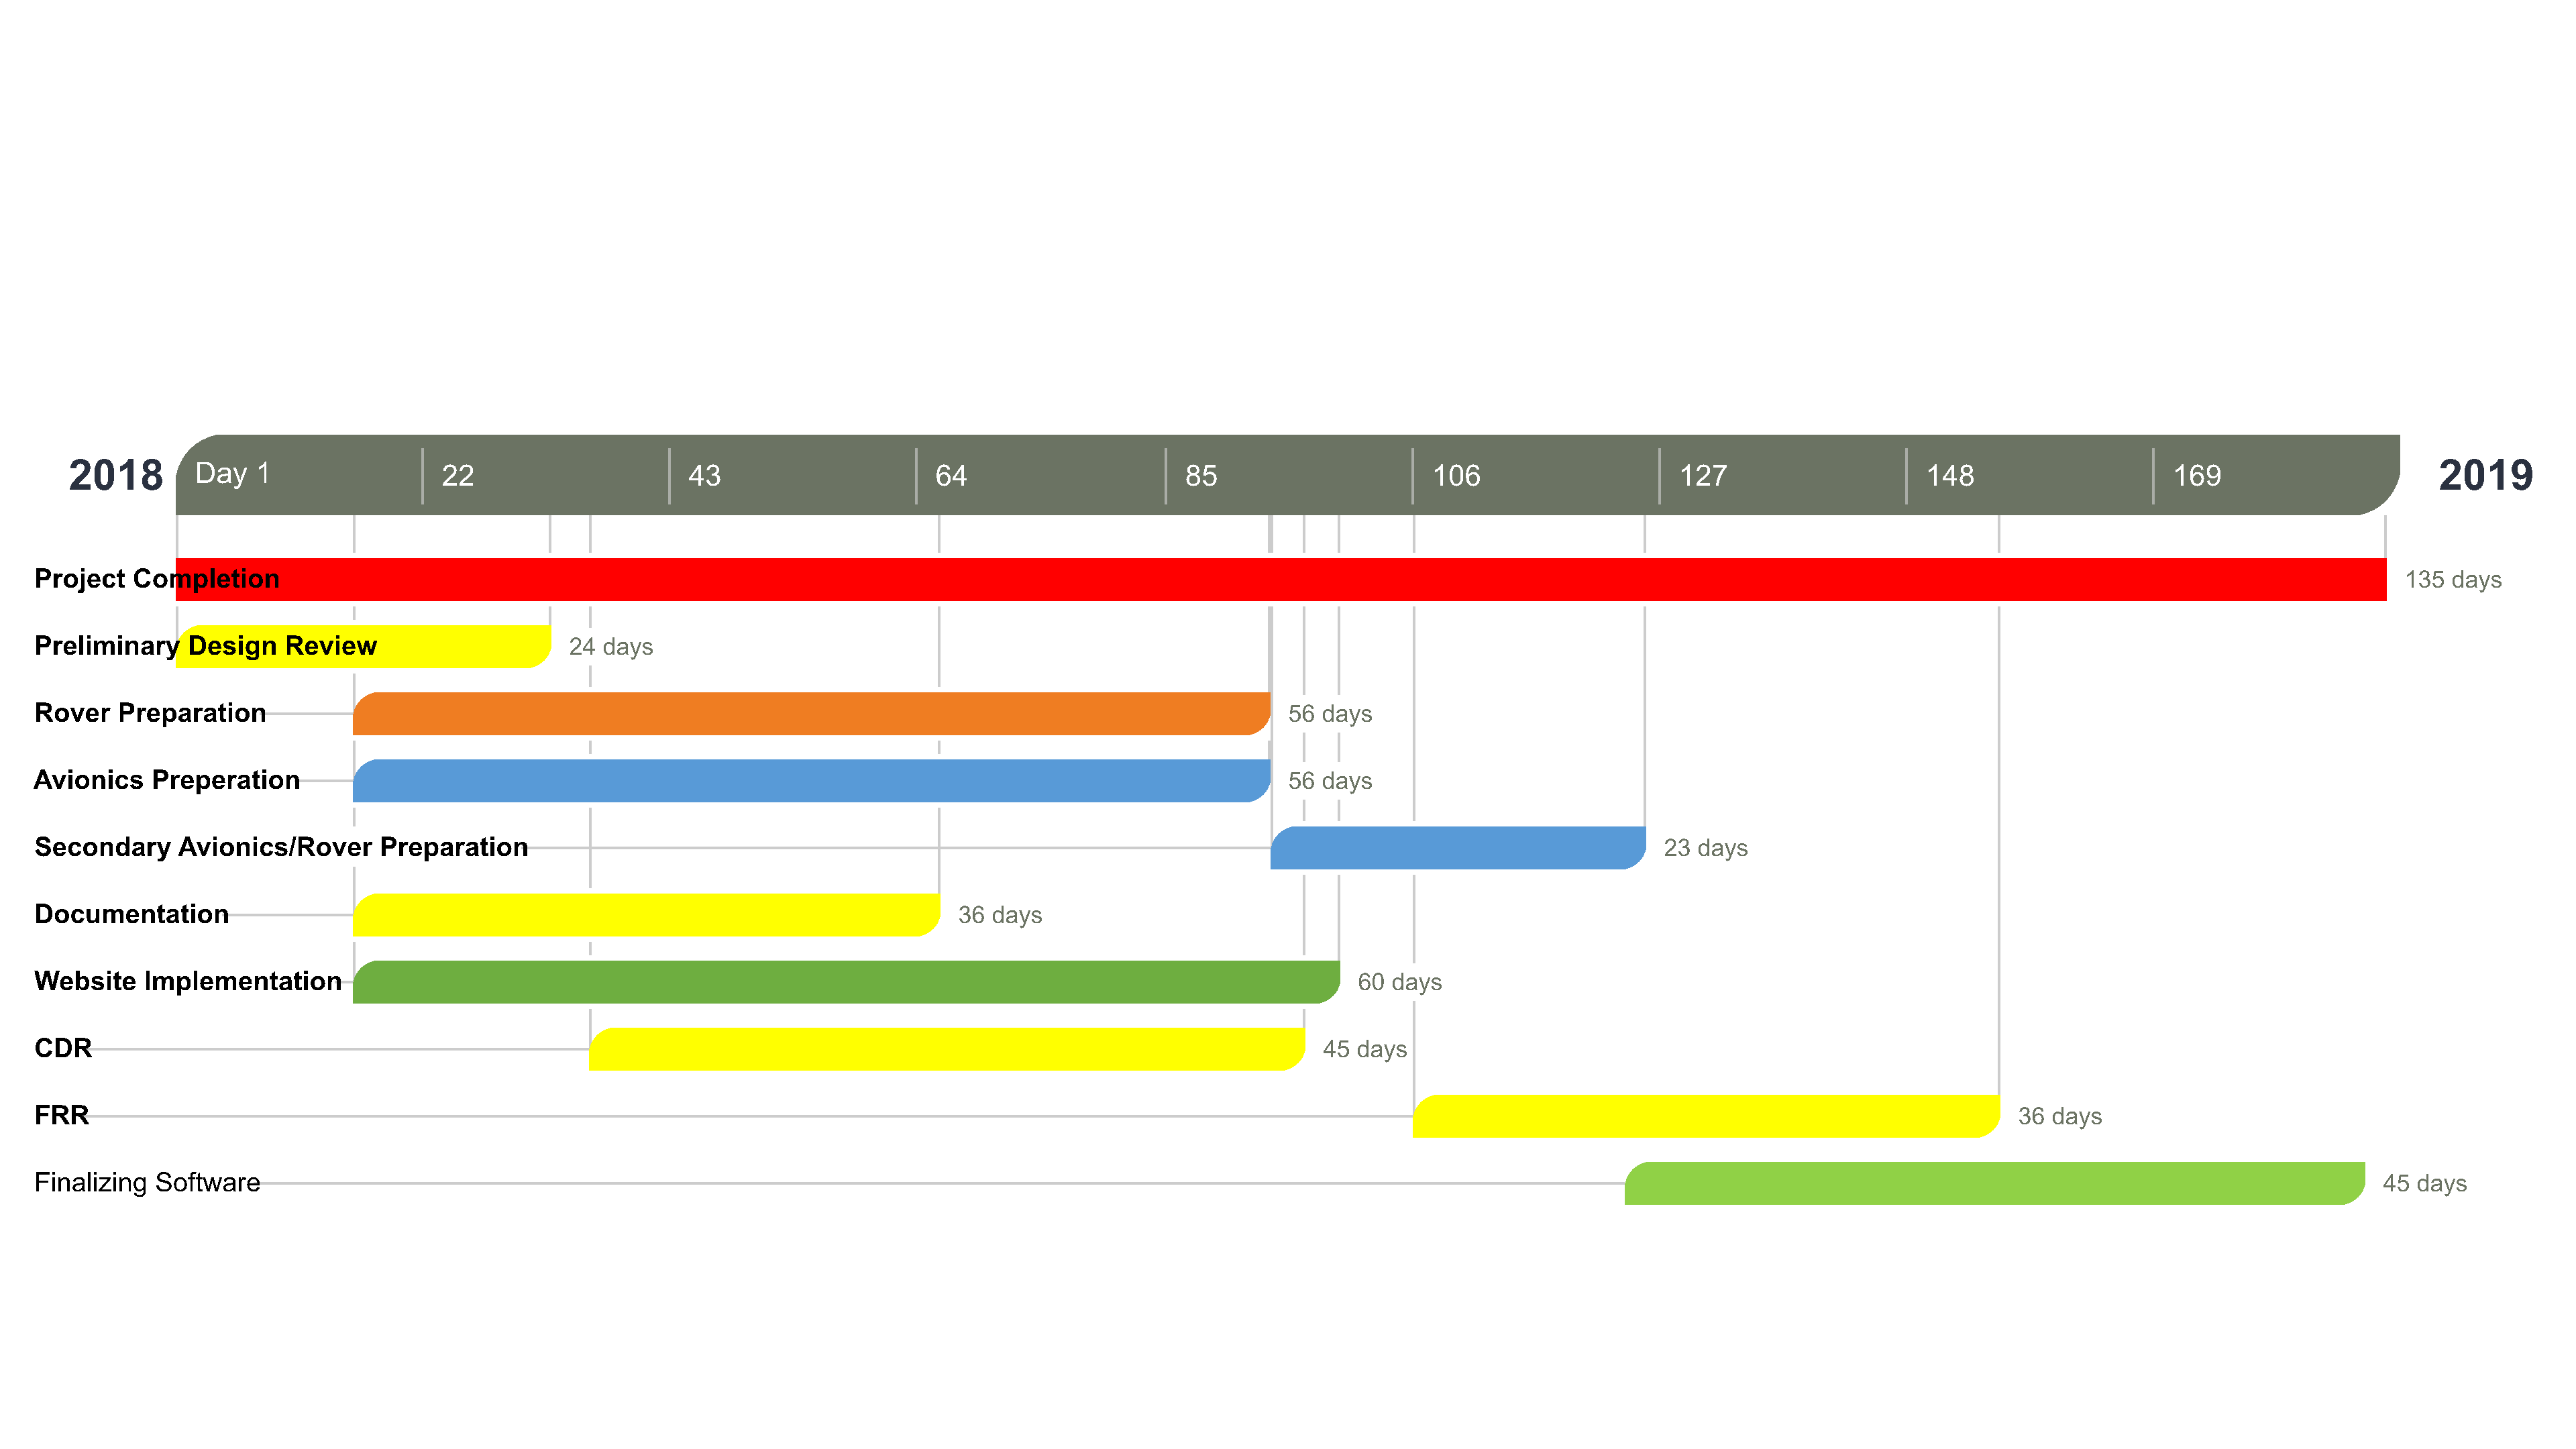
\includegraphics[width=\paperwidth]{Figures/PlanningRoadmap.png}} 
\end{center}

\newpage
%Design Document Section%
\section{Design Document}
\subsection{Revision Table}
Sections have been incremented by 1 from our drafts to our final draft because of the addition of the revision table.
\begin{table}[h]
\centering
\begin{tabular}{|l|l|l|}
\hline
Section & Original & New \\ \hline
3.1 & \begin{tabular}[c]{@{}l@{}}Object detection \\ using computer vision.\end{tabular} & \begin{tabular}[c]{@{}l@{}}Small technical changes\\ to object detection using \\ computer vision that did \\ not get implemented.\end{tabular} \\ \hline
3.2 & State Diagram & \begin{tabular}[c]{@{}l@{}}Changed State Diagram to \\ reflect final structure. Also\\ changed text to reflect these \\ changes.\end{tabular} \\ \hline
3.3 & Class Diagram & \begin{tabular}[c]{@{}l@{}}Changed diagram to show used\\ functions and updated components.\end{tabular} \\ \hline
4.2.1 & N/A & Added a beaglebone black section. \\ \hline
4.4 & N/A & Added a components section. \\ \hline
4.5 & N/A & Added a systems section \\ \hline
5.1.2 & Redux & Removed Redux \\ \hline
5.1.4 & Webpack & Removed Webpack \\ \hline
5.2 & User Use-Case & \begin{tabular}[c]{@{}l@{}}Updated User Use-Case to reflect\\ final structure\end{tabular} \\ \hline
5.3 & Admin Use-Case & \begin{tabular}[c]{@{}l@{}}Updated Admin Use-Case to reflect\\ final structure\end{tabular} \\ \hline
2.4 & N/A & Added GPS \\ \hline
3.1.1-3.2.3 & N/A & \begin{tabular}[c]{@{}l@{}}Removed 433 MHz references, more \\ info on PLEC and talked about new \\ GPS system.\end{tabular} \\ \hline
3.3 & N/A & Removed references to 433 MHz system \\ \hline
3.4 & N/A & \begin{tabular}[c]{@{}l@{}}Modified project objectives to be in line\\ with what we actually worked on.\end{tabular} \\ \hline
\end{tabular}
\end{table}


\subsection{Introduction}

\sffamily

\subsubsection{Purpose}
The purpose of this document is to define software systems in order to give the team an overall understanding of the design of each component. This will provide our sub-team and the entirety of the USLI team insight into the topics covered throughout the implementation of the project.

\subsubsection{Scope}
The avionics, payload, and website will be utilized to compete in a competition hosted by NASA. The mission consists of a single-state solid propulsion rocket being launched to a target altitude of about one mile. At apogee, the rocket separates into 2 sections and safely touches down on the ground using an integrated recovery system. The avionics system tracks the location of the launch vehicle for the duration of the flight. After landing, the aft section of the rocket ejects a robotic payload that must move at least 10 ft. from the rocket body, collect a soil sample with a minimum volume of 10 ml, and then store the sample in a sealed container on-board the payload. Once collected, the sample will be taken to a base station for analysis. The base station analysis is not a part of the NASA competition, but the team decided to pursue it to add scientific value to our entry. Furthermore, the team must develop a robust website to deliver technical documents to NASA and display team information and educational outreach efforts.

\subsubsection{Context}
The mission will utilize programming languages and software utilities to provide commands and control for the hardware devices - namely micro-controllers such as the Teensy 3.6 - that will comprise the computational systems integrated into the launch vehicle and robotic payload. We will use ReactJS and Material-UI to design and build a website that is capable of delivering technical documents and technical information about the team. The usage of these hardware and software components combined will provide the necessary modules and deliverables for execution of the team's entry for the 2019 NASA Student Launch Initiative Competition.  
\subsubsection{Glossary}
\begin{itemize}
    \item \textbf{ATU} - Avionics Telemetry Unit: a series of micro-controllers, sensors, and transceivers that collects, transmits, receives, and logs data during rocket flight.
    \item \textbf{CV} - Computer Vision.
    \item \textbf{GPS} - Global Positioning System. One of several worldwide navigation satellite networks used in commercial navigation technologies.
    \item \textbf{NMEA} - National Marine Electronics Association, a standardized format for positional data that is widely used by GPS and other positioning systems.
    \item \textbf{PLEC} - Payload Ejection Controller, receives signal from the ATU ground station to fire off black powder charges and eject the robotic payload from the launch vehicle aft.
    \item \textbf{ReactJS} - A JavaScript library to provide user interfaces through small scripts known as 'components'. Will be used in concert with the Material-UI library. 
    \item \textbf{USLI} - University Student Launch Initiative, a yearly competition hosted by NASA in which university teams compete to build, launch, and operate a rocket and scientific payload. Frequently used to reference the OSU competition team itself.
\end{itemize}

\subsection{Avionics}
The Avionics Telemetry Unit (ATU) is responsible for the generation, logging, filtering, transmission, reception, and output of position and telemetry data while the rocket is in flight. The ATU assists in recovery of the rocket components after launch and collects data which is analyzed via software (MATLAB scripts that are not a part of our capstone project) after the flight to extrapolate critical launch data. The avionics system is composed of a ground station and a pair of flight units that communicate wirelessly using a custom packet system during the flight. The flight units collect and transmit the avionics data to the ground station during the flight. The ground station transmits the received flight data to a USB-connected computer that outputs the data over the Arduino serial monitor. The ground station is also responsible for transmitting an ejection signal to the Payload Ejection System (PLEC) once the rocket has landed and is ready to eject the rover. Modularization and functional decomposition of the code for both systems facilitates ease of development and adaptation.

\subsubsection{System Design}
The avionics system is composed of a ground station and multiple flight units that are placed within the rocket. Each has its own hardware and software components, and the system as a whole works together to ensure the mission profile is met successfully.

\paragraph{Flight ATU}
The Flight ATU is composed of a GPS module, Teensy 3.6 ARM micro-controller, XBee Pro S3 900 MHz transceiver, and an antenna which are all embedded and connected on a custom PCB created by USLI electrical engineers. The GPS module receives positional data from various navigation satellite networks which it then transmits to the Teensy as NMEA (National Marine Electronics Association) formatted packets via serial communication. The Teensy writes all of the given NMEA-format packets to the on-board SD card, then uses a C/C++ program to discard all non \$GNRMC-type packets, strips unnecessary information out of the \$GNRMC packets, and packages them into a new packet format which is sent over serial to the XBee Pro transceiver module. The custom packet structure has the following information (and more) added to it:

\begin{itemize}
    \item Custom start delimiter - 0x7E
    \item Least and most significant bits for delimiting at the beginning of the packet
    \item Frame type (TX/RX Request)
    \item Frame ID Number
    \item 64-bit Target Address (currently hard coded)
    \item Reserved bytes
    \item Transmit options
    \item Checksum
\end{itemize}

\paragraph{Ground Station ATU}
The ground station ATU is very similar to the flight ATU, but boasts a different set of code on the Teensy, a larger antenna, and the capability to connect to a computer via serial (USB). The XBee Pro receives the packets from the flight ATU and sends them via serial to the Teensy. If the Teensy detects a packet in the serial buffer, it loads the packet, unpacks it, determines which ATU (of the 2 flight units) it came from, then pipes the data out over the serial interface with the computer. The ground station also boasts a button and switch which are used as safety controls for the payload ejection control signal; both must be activated simultaneously and the trigger code must be flashed for the signal to broadcast.  \newline

\subsubsection{Design Rationale}
A majority of the design decisions made for the avionics system stem from decisions made during last year's software and electrical engineers. This year, the goal is to modify the embedded avionics code to be at least 25\% shorter, correctly commented, and functionally decomposed (rather than 2-3 large functions, as it was last year). We also want to fix the code for the PLEC and integrate it more effectively with the ground station, and ensure that the avionics code can be ported to a new custom PCB with a new GPS unit.

\paragraph{Micro-controller}
The Teensy 3.6 was determined to be the most effective micro-controller for both ATUs due to its speed, size, and ease of programming. The Teensy 3.6 has a clock speed of 180 MHz - more than 11 times faster than the 16 MHz processor on a standard Arduino Uno. This makes the Teensy superior for high speed embedded applications with significant data throughput. The Teensy lacks many of the components that many other consumer micro-controllers are shipped with - ex. non-USB power input, large LEDs, heatsinks, pin headers, etc. - giving it an advantageously small power and spacial profile. Support for serial communication and the ability to write to an on board SD card are also critical functionalities that the Teensy offers. A micro-controller was chosen over a small embedded PC such as a BeagleBone or a Raspberry Pi due to the detrimental effects that software overhead such a system inflicts on the data transmission and receiving process.

\paragraph{GPS}
The old GPS unit was replaced with a UBlox GPS unit with increased compatibility with global navigation satellite systems. The old GPS chip only interacted with the American GPS network, but the new chip can interact with GLONASS, BeiDou, and Galileo. Hardware differences mandated a change in programming and the serial communication protocol in order to accommodate the new keywords utilized by the NMEA format for satellites that aren't on the American GPS network.

\paragraph{Transceivers}
The XBee Pro S3 900 MHz transceiver is the current de facto Rx/Tx device in the system due to ease of implementation with pre-existing libraries from the manufacturer, the ability to transmit on the 900 MHz band without a commercial license, and the relative power and range that a 900 MHz transmission band offers. The current 900 MHz system is capable of and tested for reliable packet transmission within a 2 mile line of sight distance at 250 mW of power on a high gain antennae; transmission will be at either 210 mW or 250 mW depending on the other transceiver system's power output to keep our signal emission within a reasonable operational range. The competition rules stipulate a combined outgoing signal power of 250 mW as the cap for operation.\newline

\noindent Unfortunately, the 900 MHz band is prone to interference due to its popularity as a license-free consumer radio frequency. The USLI team experienced technical difficulties last year due to the presence of multiple other higher powered RF transceivers operating on the 900 MHz band at the competition. Since the launch vehicles must be set up and wait for a given duration of time, the 250 mW transmission was easily overpowered and data integrity was significantly impeded.\newline

\noindent To combat the problem of interference on the 900 MHz band, the USLI team would like to put together a very basic functioning proof-of-concept prototype of a 433 MHz radio-frequency communication system. 433 MHz transmission offers relatively high data fidelity, a range encompassing the expected flight and landing distance of the rocket, and its infrequent use due to its restricted band status makes it highly unlikely that any interference would occur from other devices on the same frequency. The hope is that such a system can be expanded upon by subsequent teams in order to overcome the shortcomings of the 900 MHz system. The main drawback to using 433 MHz transmission is the lack of modular and ready to use consumer grade radio frequency devices. The USLI team will not be implementing a full 433 MHz system this year due to shortages of personnel, time, and team resources.

%% Trey

\paragraph{Programming Languages}
AVR compatible C and C++ are the languages of choice for the Teensy and embedded control code; no other high level languages are easily implemented with the given micro-controllers, and AVR assembly is too difficult to reasonably implement without tackling a steep learning curve that the team doesn't have time to address. Furthermore, C and C++ have their own well fleshed-out standard libraries and are compatible with Arduino and XBee Pro libraries. Some MATLAB is also being used to interact with the data that the avionics system generates, but the scripts are already mostly developed and its operation doesn't fall within the jurisdiction of our capstone project.

\newpage
\subsubsection{Diagrams}
\vspace{1cm}
\begin{figure}[ht]
    \centering
    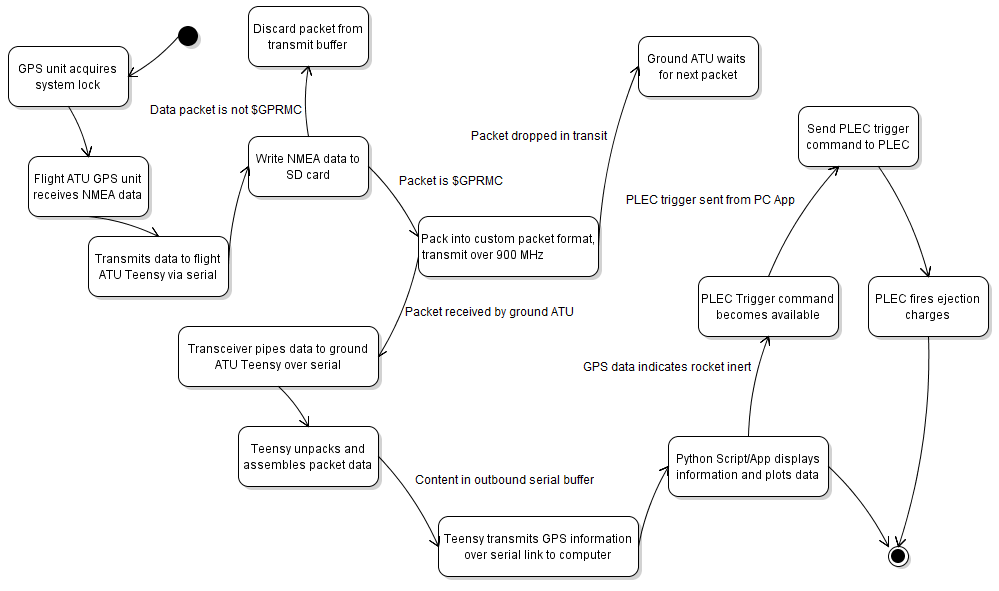
\includegraphics[width = 0.9 \textwidth,angle=0]{Figures/avionicsStateDiagram.png}
    \caption{Avionics State Diagram}
    \label{fig:Avionics SD}
\end{figure}

%\vspace{1cm}
\begin{figure}[ht]
    \centering
    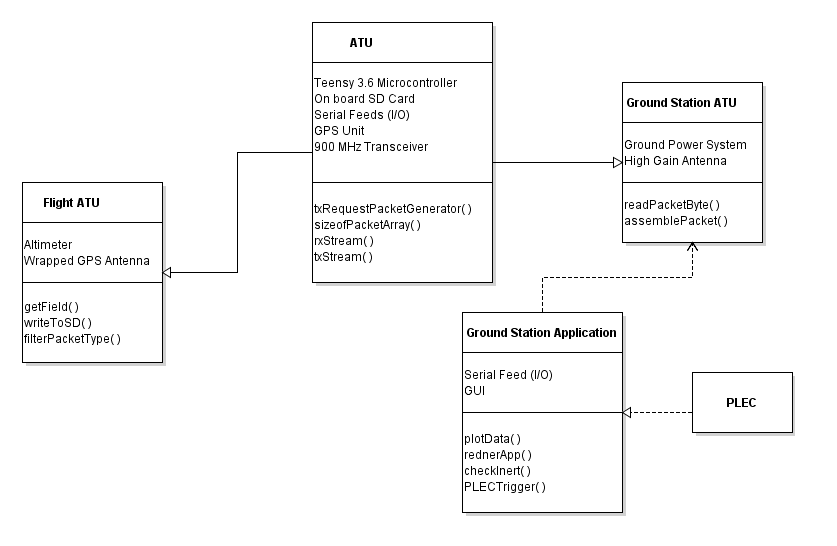
\includegraphics[width = 1 \textwidth,angle=0]{Figures/ATUclassDiagram.png}
    \caption{Avionics Class Diagram}
    \label{fig:Avionics CD}
\end{figure}

\newpage
\begin{figure}[ht]
    \centering
    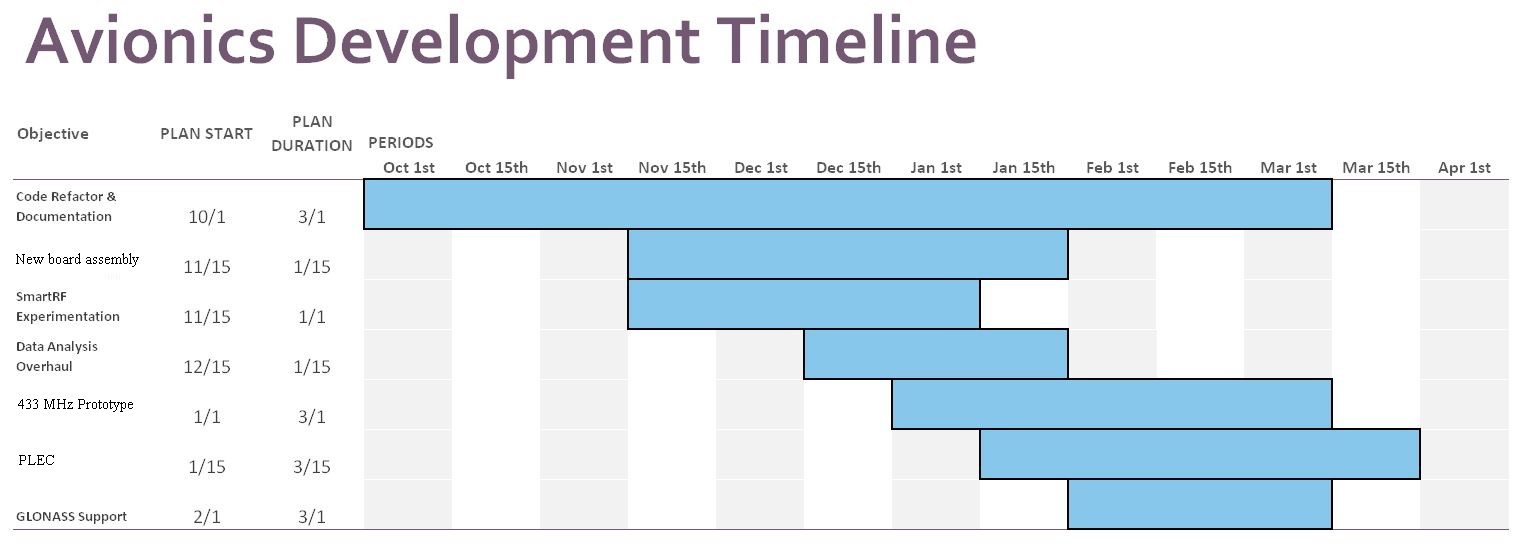
\includegraphics[width = 0.95 \textwidth,angle=0]{Figures/ganttATU.JPG}
    \caption{Avionics Gantt Chart}
    \label{fig:Avionics Gantt}
\end{figure}

\newpage
\clearpage

\subsection{Payload}
The payload will be responsible for a large majority of the mission after ejection. All tasks must be completed while remaining completely autonomous. The tasks that must be completed are the following:

\begin{itemize}
    \item Travel at least 10 meters from any part of the rocket
    \item Find a desirable location to collect a soil sample
    \item Activate auger to collect soil in a sealed container
    \item Receive GPS base station coordinates
    \item Travel to the GPS coordinates sent to the rover
    \item Dock to deliver soil sample that will be released from the rover
    \item Standby to collect and deliver additional samples to the base station
\end{itemize}

\setlength{\parindent}{0cm}
In order to complete the above tasks, the rover must be pre-programmed with a complex set of instructions to follow. The rover will continuously be taking in data from the environment using a camera and sonar sensors to check for obstructions and have the required intelligence to successfully avoid obstacles and remain on track to the destination. The rover is equipped with a GPS in order to guide the robot away from the rocket body to achieve the minimum distance from the rocket body as well as guide the rover to the base station in order to deposit the samples. A gyro will let the rover know if the area being drilled is feasible to obtain a soil sample and if the gyro is within operating range for the auger. The motors must be capable of quickly maneuvering around and over terrain. The rover must have an RF receiver to receive GPS coordinates from the rocket body and the base station for navigation. After the rover obtains the coordinates of the scientific base station, a routing algorithm using GPS and the magnetometer for the heading will guide the rover to the base station for soil sample delivery. 

\subsubsection{Design Viewpoints}
Practicality was taken into account during the design phase of the rover. The program on the robot will need perform autonomously, so there is no room for error. As such it has been designed with every situation in mind in order to not  become stuck in any specific process. For this reason, there exists an extra computer attached which will be in charge of computer vision. This computer will be responsible for communicating with the Teensy on the rover and giving instructions to follow for docking at the base station. Due to the separation of hardware, the rover would be able to complete the mission even on destruction of non-critical components during ejection (i.e. the BeagleBone - located outside the chassis of the rover). 

\newpage
\begin{landscape}
\subsubsection{State Diagram}
\vspace{1cm}
\begin{figure}[ht]
    \centering
    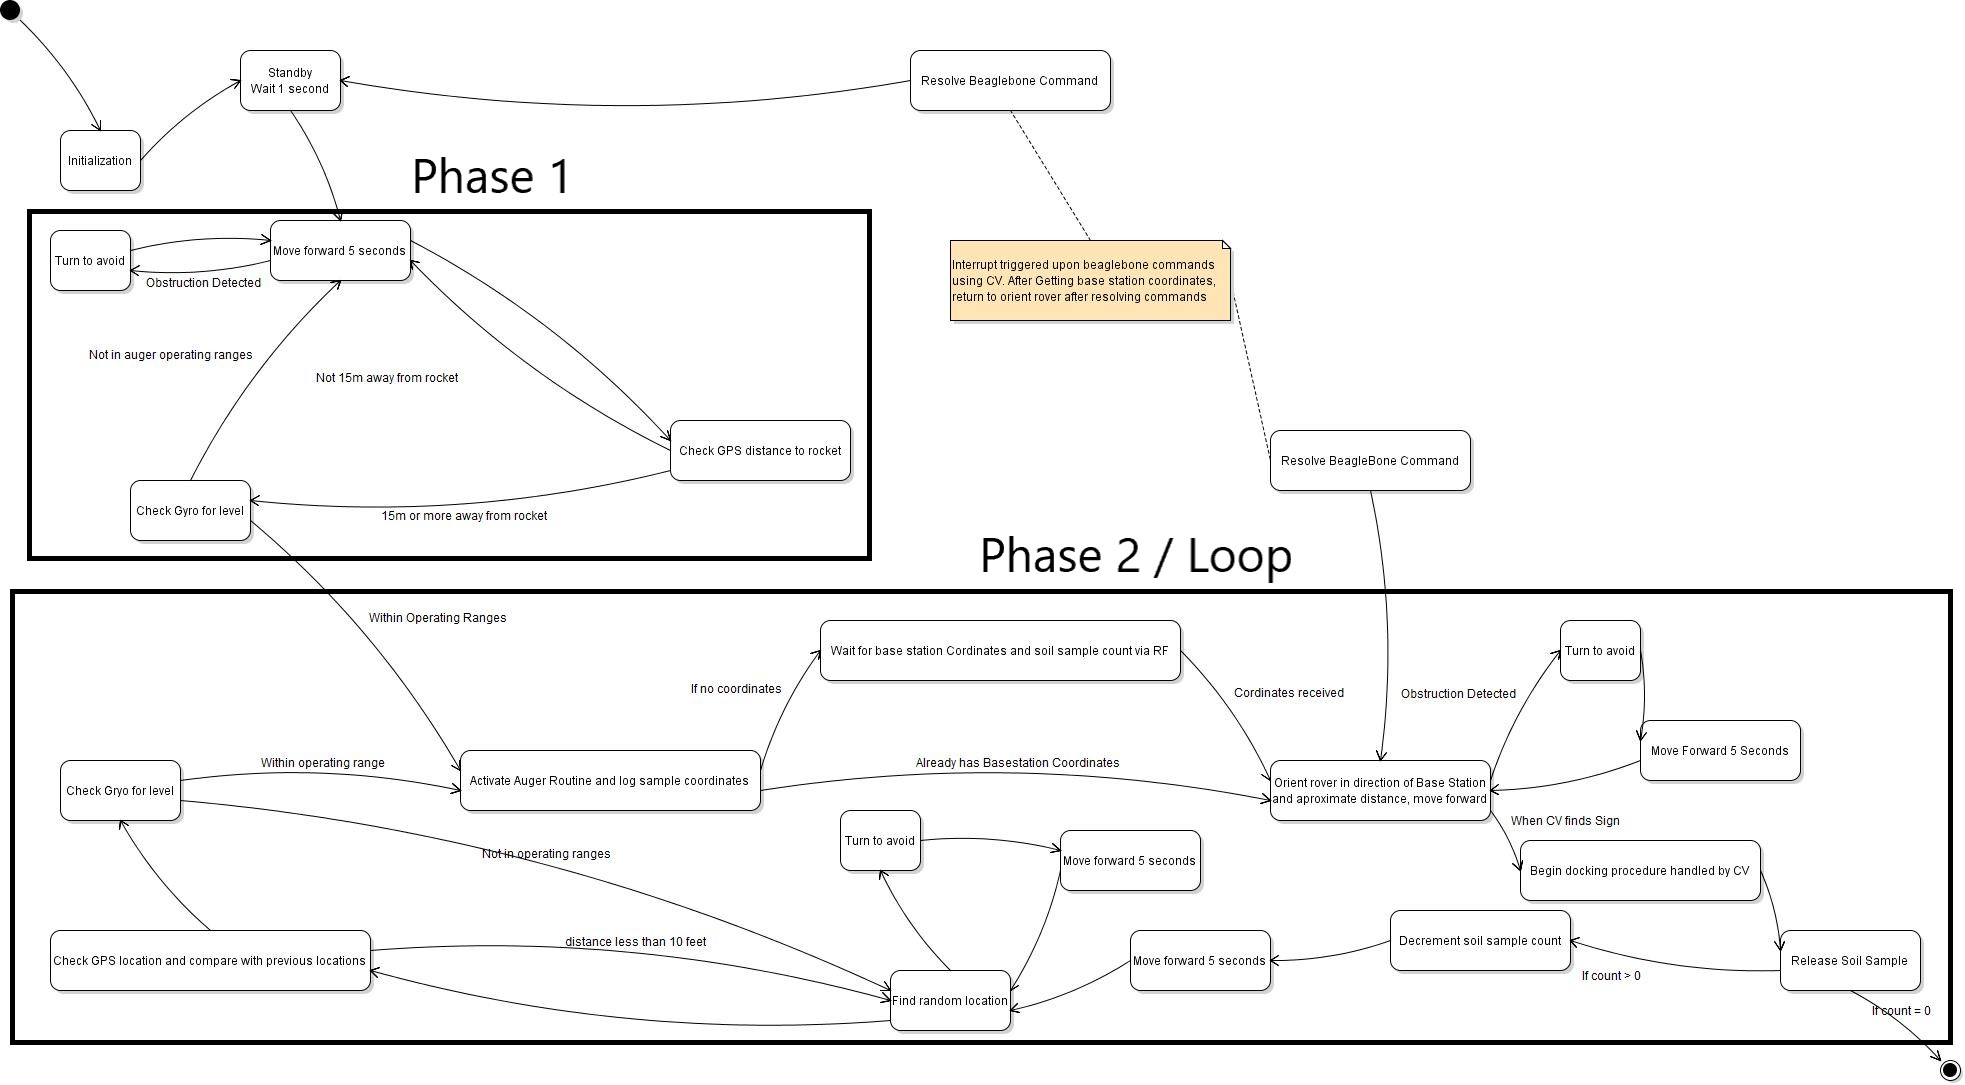
\includegraphics[width = 1.3 \textwidth,angle=0]{Figures/TeensyStateDiag.jpg}
    \caption{Rover State Diagram}
    \label{fig:my_label}
\end{figure}
\end{landscape}

\newpage
The state diagram shown above (figure 1) begins after the payload is ejected from the rocket body. The rover begins by initializing when the rover obtains the GPS coordinates of the rocket. The rover will then start phase 1 of its programming. This involves the rover moving forward until it is at least 10 meters away from the rocket while practicing object avoidance and then finding a level spot to collect a soil sample. The distance between the rocket and the soil sample is verified using GPS. After the soil sample has been collected, the rover freezes and waits for a GPS coordinate that will begin phase 2. During phase 2, the rover will begin to deliver the soil sample to the base station using GPS routing algorithms. The rover will travel in the direction of the base station while continuously avoiding obstacles. After the rover is in close proximity of the base station, it will begin searching for a target on the base station using CV. When the target is found, the rover will be fed instructions by the BeagleBone on how to move in order to climb a ramp for the base station. The BeagleBone is able to find the target and transmit the location to the Teensy effectively. Due to insufficient testing time, fine tuning for docking was not completed. After the rover successfully climbs the ramp and finds its way to a level surface at the top, the rover will check the gyro for level ground and release the soil sample on the level surface. After the sample has been delivered, the extra base station activity will be complete. If extra samples are required the rover will continue on back down the ramp in order to fetch more samples. The number of samples are specified during transmission of the base station location.

\paragraph{BeagleBone Black}
The BeagleBone is programmed using OpenCV 3 to detect for circles with a Hough Circle transformation after the image grabbed is processed through a grey-scale and canny filter in order to look for hard lines. These lines are fine tuned in a way such that they will not detect false positives. This is done by only allowing edges to be drawn for images with black on white. For this reason a black target on white paper is used. This was to circumvent the possibility of triggering false positives on objects such as tractor wheels that might be on the farmlands of the launch site. The image is then processed and fine tuned to only detect on a strong correlation to a circle that would be found on the target. As a result the BeagleBone was able to consistently detect the target while having very few false positives even in the worst environments. The target was tested to a 45 degree angle while still consistently detecting the target. After the circle is detected, the center point of that circle is then converted into a certain number of pixels left or right of the center of the frame. An instruction for each detected frame is fed to the Teensy over UART in an instruction that looks like "L-1!" or "R-640!". This gives the Teensy measurements to work with to determine the amount to turn in order to climb up the ramp. The Beaglebone is able to run at 0.3 frames per second while a target is recognized or 0.7 frames per second while no target is found. A resolution of 720x1280 was chosen as to get the maximum accuracy and range while not slowing down the frame rate more than necessary. 

\newpage

\vspace{0.5cm}
\subsubsection{Component Diagram}
\vspace{1cm}
\begin{figure}[ht]
    \centering
    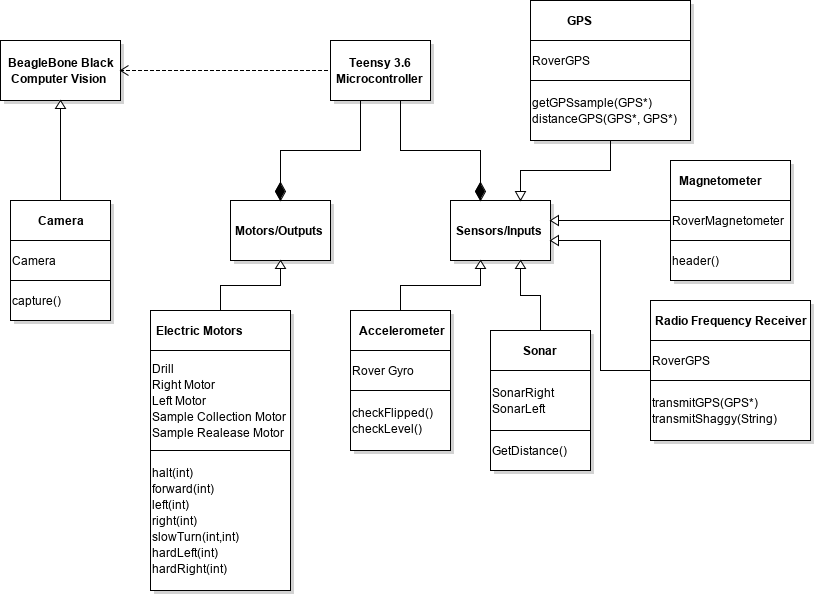
\includegraphics[width = 1 \textwidth,angle=0]{Figures/ClassDiag.png}
    \caption{Rover Component Diagram}
    \label{fig:my_label}
\end{figure}
\vspace{1cm}

This class diagram shows the relation of the different components and sensors to the Teensy micro-controller and BeagleBone computer. It shows what hardware will be used and what commands may be used to interact with each device. These devices will be implemented with the functions for controlling each piece of hardware on a lower level. This will help organize the code into a modular arrangement where devices can be called as they are needed for the rover's programming. The BeagleBone is connected to the Teensy as it will be sending interrupts to call specific routines that will be pre-programmed onto the Teensy. Connected to the BeagleBone is a camera that will be able to take a frames to process of the area in front of the rover throughout program.

\subsubsection{Components}
\paragraph{Motors}
The motors will be controlled with multiple functions that will set the motors to specific power levels relating to the input that they have been given. The motors use power values between 0 and 255. Each function steadily changes the power by 1 each 10 milliseconds so that the motors do not take any damage and the rover will not tip over from an abrupt stop. Many of the functions are self explanatory: halt will stop the rover, forward gets the rover moving forward. The left and right function cause the rover to move right or left by the movement of 1 wheel while the other wheel is stopped. The hardRight and hardLeft functions however are a little different; These functions cause the rover to turn half the power (given by the parameter) reverse for one wheel and power equal to the value forward for the other. 

\paragraph{Accelerometer}
This device is used functionally as a gyroscope. When the rover is stopped, the gyro can be read in order to see the direction gravity pulls. The gyro is perpendicular to the ground and thus can be used to find level ground. The accelerometer has two custom functions. checkFlipped will return true if the rover is flipped and checkLevel will return true if the rover is sufficiently close to level.

\paragraph{Sonar}
These devices are capable of detecting objects in a cone in front of the rover as well as the distance in front of the rover that the object is. A sonar is located on the left and right of the rover which can be used to identify which direction to turn. The getDistance function reads from the sonars giving a value from 0.2 to 5 meters. If no object is located in front of the rover 5 meters is returned. 

\paragraph{Radio Frequency Receiver/transmitter}
The rover has an XBee antennae on board in order to send transmissions to a partnered antennae which is named Shaggy. This is used to send and receive transmissions from the rover. The main function required for this device is the transmitShaggy function. The project has multiple XBees so the transmission is packetized and de-packetized in order to send the message to a specific XBee, in this case Shaggy.

\paragraph{Magnetometer}
The magnetometer is responsible for detecting the earths magnetic field. The heading function call works like a compass giving a readout between 0 and 359 in degrees. This is used by the routing algorithms in order to keep the rover traveling the correct direction. The magnetometer is shielded underneath by MuMetals which act to keep the electromagnetic fields from the rover and proto-board from interfering with magnetic field readings. 

\paragraph{GPS}
The GPS system establishes lock in approximately 2-3 minutes without interference. This is read as a \$GNRMC formatted instruction and parsed with a regex in order to make a GPS object that is used many times throughout the rover mission for calculations and data recording. The distanceGPS function is an algorithm that reads the distance between two GPS objects that are passed in. Another function was also created in order to find the heading required to navigate from one GPS coordinate to another. Two GPS routing algorithms were created. The first of which is to move toward the GPS coordinate by calculating a heading and comparing that value to the value given from the magnetometer. The other is to move away. This reflects the point to move away from over the rover and multiplies that number by 5. This will insure that the rover is always moving away from that point. 

\subsubsection{Systems}
\paragraph{Soil Collection}
The soil collection system consists of an auger and a collection chamber with a top door and a bottom door. The auger and collection doors all have encoders in order to precisely measure the number of rotations each motors have taken. This is important because the door needs to open half way and close by reversing the same number of rotations to guarantee that the soil sample is sealed. More importantly the auger has a decoder in order to travel the correct distance while drilling into the earth. If the motors were to spin too far the auger enclosure would be destroyed by the motor. Using a decoder, the number of rotations down can be calculated and the reversed rotations back up can precisely rotate the same number of times back up so any offset can be prevented for the next soil sample. 

The code counts the number of rotations made by the auger and doors using interrupts. For each rotation on the way down, a pin is raised high and a counter is incremented. When that number reaches a specified amount, the counter is reset and can be rotated the opposite direction the same number of times. 

\paragraph{Object Avoidance}
In order for the object avoidance to be active at all times, the Teensy 3.6 is multi-threaded using a modified teensythreads library. The threading is possible with time division between the main thread and side thread. The main thread is set to run for 100 milliseconds and switch to the "sonar watching" thread for 50 milliseconds. The sonar watching thread is set to watch and trigger an interrupt to itself whenever either one of the sonars detect an object within 0.8 meters. When the teensy is interrupted, a function for avoidance is run and causes the rover to hardRight or hardLeft in the direction indicated by which sonar has been triggered. As soon as the object is no longer detected, control of the rover is passed back to main and the threading will continue. Object avoidance is disabled by suspending the sonar watching thread during times it is not needed and restarted after the task has been complete. 

\newpage
\begin{landscape}
\subsubsection{Gantt Chart}
\vspace{3cm}
\begin{figure}[ht]
    \centering
    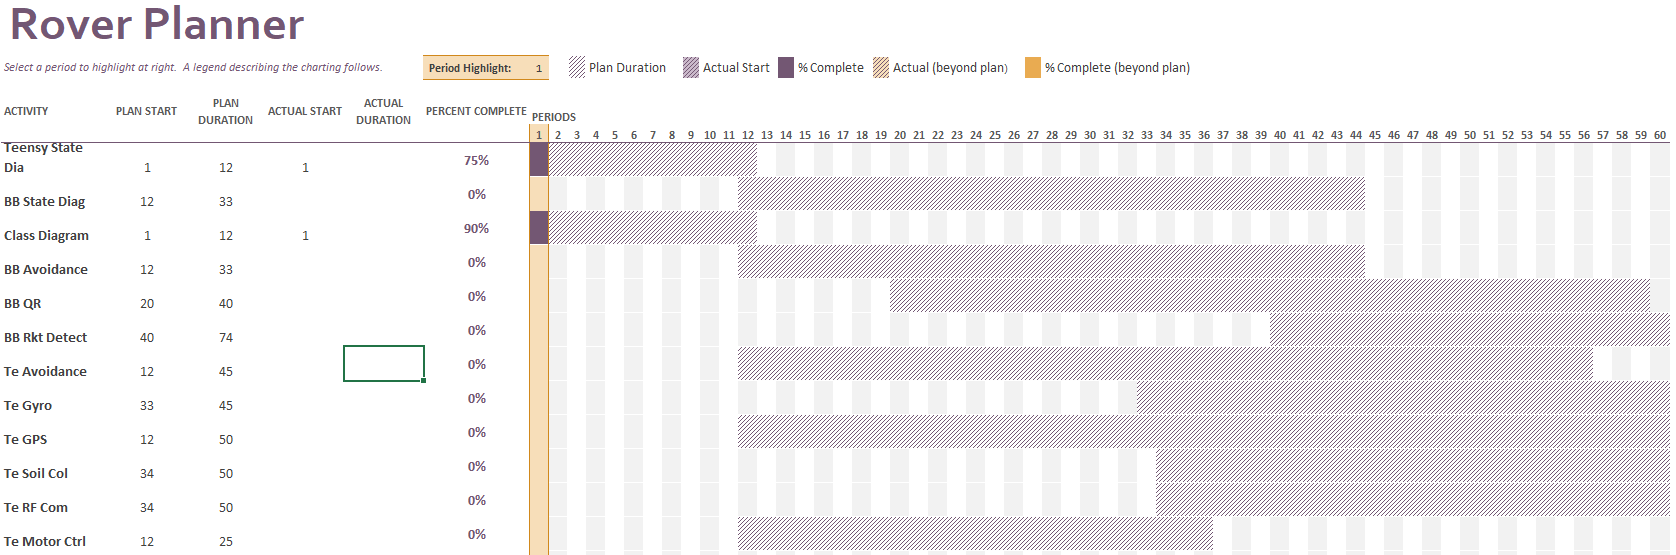
\includegraphics[width = 1.3 \textwidth,angle=0]{Figures/PayloadGantz.PNG}
    \caption{Payload Gantt Chart}
    \label{fig:my_label}
\end{figure}
    Each period will account for 1 day and the first period began on November 28, 2018
\end{landscape}

\newpage
\subsection{Website}
The website is the central location for the storage of critical documents for NASA to retrieve, one of the key social media presences for the OSU USLI team, and a location that sponsors can easily access to learn more about our team. In order for this to be created the the following will be implemented: 
\begin{itemize}
    \item React JS
    \item Redux
    \item Node.JS
    \item Webpack
    \item Browser Sync
    \item Babel
    \item Material-UI
\end{itemize}
Although the website is not directly a part of the competition, creating a website is crucial to the team's success. The website will be aesthetically pleasing, easy to navigate, and easy to access. React is also used because of the versatility with regards to mobile development.  

\subsubsection{Technologies Implemented}
\paragraph{ReactJS}
ReactJS is an open-source JavaScript used to build user interfaces specifically for single page applications. The purpose for development was to handle the viewer layer for web and mobile applications. React allows developers to create large web applications which can change data and interfaces without reloading the page. React is also fast and simple. This allows our development team have the tools it needs in order to meet the goals set by the USLI team. 
\paragraph{Node.JS}
Node.js is a an open-source environment that executes JavaScript code outside of a browser. Developers use Node.js for client-side scripting. Node.js allows developers to run scripts server-side to produce web page content before the page is sent to the user's web browser. Our team is using Node.js on our website so we can run multiple tasks simultaneously. This also meets the team's goal of efficiency. 
\paragraph{Browser Sync}
Browser Sync will be a crucial tool that the team uses for testing. Browser Sync makes changes and testing faster by synchronizing file changes and interactions across many devices. This feature is called Live Reloading and makes the page auto-reload when changes in code are made. This is implemented in the background and will help our team coordinate multiple developers while accessing and developing the new website.  
\paragraph{Babel}
Babel is a JavaScript compiler that has the following features: 
\begin{itemize}
    \item Transform syntax
    \item Polyfill features missing in target environment
    \item Source code transformations
\end{itemize}
This is also done in the backend and helps with development. 

\paragraph{Material-UI}
Material-UI is one of the most used user interface libraries for React. Material-UI has React components that implement Google's Material Design. The following reasons are why we are using Material-UI: 
\begin{itemize}
    \item Deliver on fully encapsulated React components
    \item Customization
    \item Cross browser compatibility and accessibility
    \item Ease of learning
\end{itemize}
Material UI was used to help create the Home page, About Us section and the Deliverables. Templates and examples were given as well as support. 
All of these tools will give the team the ability to develop a website that will meet the goals set and contribute to the team's success. 

\newpage
\subsubsection{User Use-Case Chart}
\begin{figure}[!htp]
    \centering
    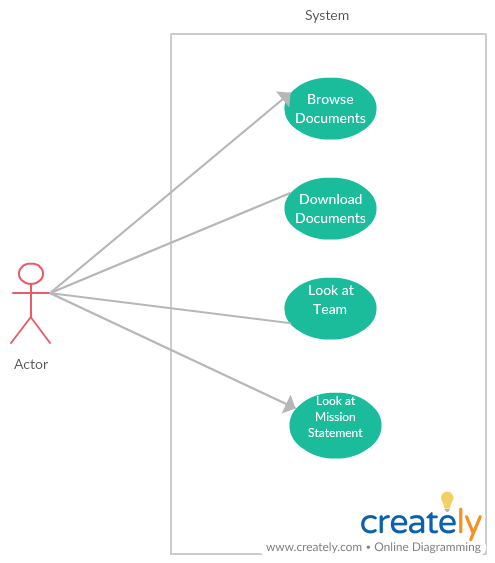
\includegraphics[scale = 0.5, width = 1 \textwidth,angle=0]{Figures/Website_User_Use_Case.png}
    \caption{Use Case - User}
    \label{fig:my_label}
\end{figure}
This figure shows what the user is able to do when they access our website. We will have an About Us section, Documents section and Home page. NASA needs to be able to download our documents that we submit for the competition so there will also be an option to download the pdfs. 

\subsubsection{Admin Use-Case Chart}
\begin{figure}[!htp]
    \centering
    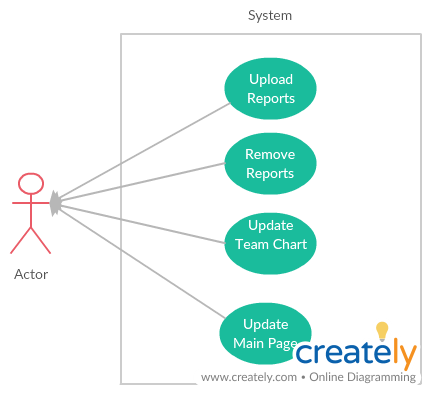
\includegraphics[width = 1 \textwidth,angle=0]{Figures/Admin_User_Use_Case.png}
    \caption{Use Case - Admin}
    \label{fig:my_label}
\end{figure}
This figure shows the options that the admin of the website has. We will have pictures of the team up so they will be able to update the website with current pictures. Admins can also update our progress, add documentation needed for NASA and update the sponsor list. 

\newpage
\subsubsection{Gantt Chart}
\begin{figure}[!htp]
    \centering
    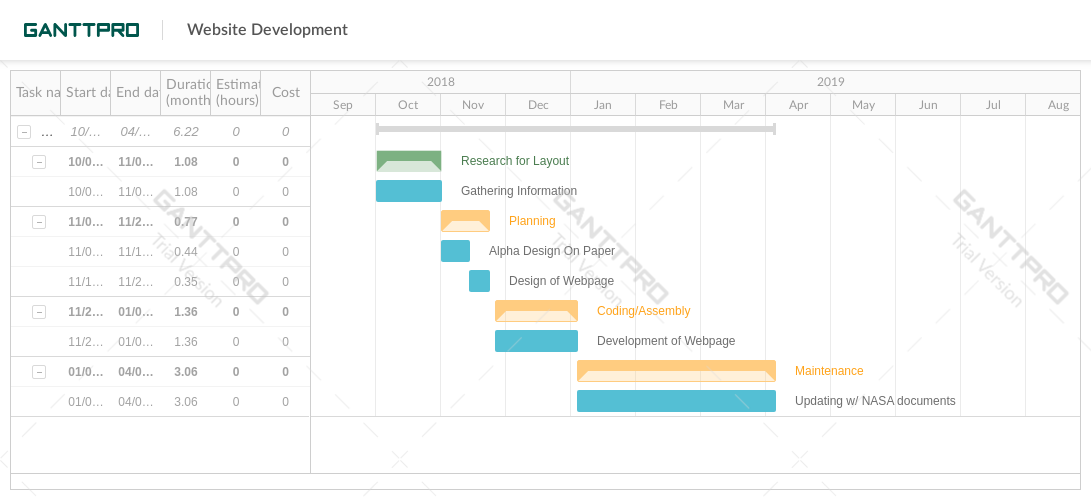
\includegraphics[width = 1 \textwidth,angle=0]{Figures/WebsiteDevelopment.png}
    \caption{Website Gantt Chart}
    \label{fig:my_label}
\end{figure}
This figure is an overview of the development of our website for the Oregon State USLI team. We must have a functional product by January 4th. This is when a critical document for NASA is due. After January 4th we will be continuing our development as well as maintenance of the website.  

\subsection{Conclusion}
This document explains and summarizes the avionics, payload, and website systems that the CS team is implementing for NASA's 2019 University Student Launch Initiative Competition. Key terms are explained, design components for each system are enumerated, and design rationale is laid out and expanded upon. The team must apportion the work appropriately, communicate effectively, and work together to deliver the required functional products for OSU's rocket launch at the NASA USLI competition in April 2019. Each system presents its own challenges and obstacles, but each system is critical to OSU's competition entry and potential victory. Care must be taken to ensure that each system is completed to requirements and expectations, and that the best products that team 12 can create are delivered to the USLI team.

%Section for Tech Review%
\section{Tech Review}
\subsection{Donald "Trey" Elkins's Tech Review}
\subsubsection{Abstract}
The following document is an analysis of the technologies that can be used to satisfy design and production requirements for the 2019 USLI software subteam. This document covers possible technical solutions for the rover payload, rocket avionics/telemetry system, and team website. Please note that some of the text is very similar to the problem statement submitted previously.

\subsubsection{Introduction}
From a high level perspective, the CS team on this year's project has three primary technical responsibilities:\medskip
\begin{enumerate}
    \item Update and maintain a team website to display progress and achievements, as well provide NASA a central location to retrieve technical documents.
    \item Ensure the rocket has a functioning avionics and telemetry system to monitor position, produce flight data, transmit data back to a ground station, and plot and analyze data. Additionally, redundancy measures must be taken to prevent signal jamming.
    \item Program an autonomous rover system that can move, avoid objects, collect a soil sample from indeterminate environmental conditions, and return the sample to a scientific base station.
\end{enumerate}
I have several personal roles on this project. From an administrative standpoint, I am serving as the subteam lead and am thus responsible for scheduling meetings, delegating development tasks, chaperoning volunteers, and making sure deliverables are completed and submitted to the team on time. From a technical standpoint, I am the primary party responsible for refactoring and adding features to the existing avionics and telemetry system used by the rocket. I am adding a second frequency band as well as updating the GUI and data analysis scripts used for the avionics system.

\subsubsection{Website}
NASA is fetching all published technical documents from the team website, and social media and web presence are a significant part of the team's competition score. It is imperative that an aesthetically pleasing and functionally robust website is developed for the team. The current site uses relatively standard HTML, CSS, and JS and is created and hosted using Github's Github.io functionality. The following are options for revamping the website presence:

\paragraph{Continued use of Github.io}
The current website is functional and requires very little maintenance work in the realm of low complexity HTML, CSS, and JS (without any notable frameworks) to get it working to team standards, but it is not particularly technically impressive or aesthetically pleasing - it gets the job done in a respectable manner and without being an eyesore. The goal is to employ something with more technical complexity and aesthetic flashiness to give NASA and other competition teams a good impression, and to measure up to the complex websites created by other competition teams in past years.

\paragraph{ReactJS}
ReactJS is a JavaScript framework created and maintained by Facebook. It is highly modular, feature packed, and well documented - making it an easy development tool that's relatively quick to learn and adopt while also making it powerful enough to create modern multimedia websites. React effectively replaces standard HTML and CSS programming with its own object structure that abstracts systems and makes them significantly more flexible and dynamic through the React API. One of our volunteers spent most of his summer working with React JS. This expertise, combined with the ease of implementation that Google's Material-UI provides, makes this the primary choice of website technology due to modularity and ease of development.

\paragraph{AngularJS}
Angular is another JavaScript framework with a significant body of documentation and the ability to implement feature heavy multimedia websites across multiple platforms. Angular is notable for the amount of time that it has been supported, its ability to compile down to vanilla JS (which React has as well), and the fact that it is actively supported by Google. The team is opting to avoid using Angular because none of our personnel have previous experience with it and it seems harder to pick up and maintain than ReactJS - it is primarily a consideration of development speed and familiarity, and Angular loses out in these respects.

\subsubsection{Avionics Transmission \& Reception}
Object tracking and data logging is crucial to recovery of the rocket and post-launch analysis. The team has need for a high efficiency, low form factor avionics and telemetry system that can track multiple rocket elements in real time, transmit data to a dedicated ground station, and save data to a local data source for later analysis via script. The most critical aspect of this system as a whole is the transmission link between the ground station and the avionics unit on the rocket in-flight.

The rocket avionics unit uses a GPS receiver to lock and track the rocket, then uses an RF transceiver to send telemetry data back to the ground station periodically for display and analysis. Choice of transceiver determines signal strength and effective range, but this is more of a consideration for the electrical engineers working on the project. The software team's primary concerns are software complexity, feature density, and ease of development. The choice of transceiver determines what software libraries are available have to work with, whether firmware or drivers must be written, and the number and variety of features that can be integrated into the system to allow more precise tracking and analysis.

\paragraph{900 Mhz XBee}
The easiest technology to use is a 900 MHz Digi XBee - a consumer grade Arduino-compatible transceiver that boasts comprehensive software libraries and a line of sight effective transmission range. Development is quick and straightforward and integrates with standard C/C++ style code employed on Arduino and other ARM based systems. The only real drawback is how common the system is: since 900 MHz is a standard commercial band, the XBee is prone to jamming or interference from other systems. Last year's USLI team actually encountered some issues with jamming due to another team using a significantly more powerful transceiver on the same band. While the XBee is cheap and easy to implement, redundancy measures must be taken to ensure that the avionics system is not dead in the air.

\paragraph{433 MHz TI CC1200}
The most effective way to circumvent jamming problems is the inclusion of an additional frequency band to the transceiver configuration. 433 MHz is a relatively common radio frequency band, but the United States federal government requires possession of a HAM radio license in order to operate hardware on it, rendering 433 MHz very unlikely to be jammed and ensuring redundancy. The team is including a Texas Instruments CC1200 RF transceiver as the second band hardware. The main downside to using this specific hardware and this frequency band is the lack of already developed software modules and libraries. There is significantly more documentation and software available for 900 MHz devices due to the band's consumer-friendly nature. The team will need to either use C/C++ or a program known as 'SmartRF' to implement network configuration, a packet system, and a faux reliable data transfer protocol for successful avionics operation.

\paragraph{TeleMega Consumer Avionics Kit}
In the event that testing and development efforts end up being unsatisfactory and it proves unlikely or impossible (with current resources) to develop firmware and a reliable data transfer protocol for the TI CC1200, the team will fall back on the usage of an off-the-shelf TeleMega consumer avionics kit that implements all of the required functionalities for the rocket system at the cost of about \$500. This is not the best option as the team will score better at the competition using a custom avionics system. Additionally, creating a custom system provides more flexibility and control over how the system works holistically. Finally, \$500 is a significant sum of money and would take a chunk out of the team's overall budget, making it preferable to develop our own system in-house.

\subsubsection{Avionics Control System}
The other critical portion of the avionics and telemetry system is the microcontroller or microprocessor used to coordinate operations between the GPS receiver, transceiver, and on-board data storage. The control device must be small enough to fit in the avionics bay, compatible with the software that used for the transceivers, and capable of quick data transmission to various components. To this end, a variety of embedded systems have been considered.

\paragraph{Arduino UNO/MEGA}
The Arduino UNO and MEGA have become the poster child for embedded devices due to their expansive open-source software ecosystem, low price, and functional ubiquity. Arduino systems provide a maximum ease of development with a minimum of cost. Unfortunately, the UNO and MEGA are relatively clunky for mission purposes and use too much space on the avionics unit to keep it compact. They are also somewhat slower and less powerful than certain counterparts. They are perfect for prototyping and development thanks to support of C/C++ style of code, but the team has chosen an option that fits the mission profile more effectively. 

\paragraph{Teensy 3.6}
The Teensy 3.6 provides the best fit for the mission profile. It is smaller and faster than its Arduino cousins and will fit the avionics unit as a whole more effectively. Furthermore, it supports standard C/C++ and Arduino code and can thus be developed on in almost the same manner. It has a clock speed over ten times faster than a standard Arduino UNO, making it much more suitable for multi-functionality programs - ex. gathering GPS data, packetizing information, transmitting over an RF link, and SD card storage. The Teensy packs a needed punch at with an optimal space profile.

\paragraph{Raspberry Pi}
The Raspberry Pi is worth mentioning as a control system alternative due to its sheer computational power. It is unreasonable to expect an Arduino or Teensy to perform any kind of Python or MATLAB data analysis, but something like a Raspberry Pi can collect data from the GPS receiver and the transceivers, process it in real time, and transfer the data to a connected SD card. Unfortunately, the Raspberry Pi has significant computational overhead since it has to run an operating system, and it is prone to seizing up and freezing under higher process loads, making it a questionable choice for a control system this complex.

\subsubsection{Conclusion}
In accordance with design requirements, the team is deciding to replace the current website with a ReactJS based site, use both a 900 MHz and 433 MHz transceiver on the avionics unit, and operate the avionics control system with a Teensy 3.6 board. With the given technologies, team familiarity with them, and the available resources, these are the most effective design decisions and will be the most conducive to completion of the project and satisfying customer and competition requirements.

\subsection{Leif Tsang's Tech Review}
\subsubsection{Introduction}
In order to implement the use of object avoidance and navigation, we must use a language that best fits the purpose of our rover, allowing for a smooth development stage and high performance. The chosen method of navigation must allow our payload to perform a series of tasks that will ultimately allow the payload to deliver a soil sample to the target base station. On top of the use of computer vision for some navigation options that we can also use for object avoidance, we must also have a redundant, simpler, object avoidance system in place. This is where our sonar, connected through the Teensy 3.6, comes into place. We use one of the three provided sonar configurations in order to provide the best performance with the lowest possible overhead for space and power constraints. 

\subsubsection{Sonar Configuration for Obstacle Avoidance}
\begin{itemize}
	\item  Horizontally Inline Dual Sonar – The Horizontally aligned sonar configuration consists of a sonar module on the right and a sonar module on the left with both forward facing and approximately 8 inches apart from one another. This configuration has a great horizontal area of detection but falls flat when it comes to the third dimension in the vertical axis. The rover will have no way to differ an obstruction from a raise in elevation that can be easily climbed over. As a function of this, other unreliable methods of detecting and overcoming these obstacles will take place to compensate. This approach is not recommended.
	\item Vertically Inline Dual Sonar – This configuration will provide one sonar on top of the other sonar, both forward mounted, with approximately a 3 inch gap between the two vertically aligned sensors. This configuration, similarly to the Tri-mounted sonar, can calculate the incline of oncoming slopes but falls short in its ability to see peripheral objects along the path that can be hazardous to the rover’s mission.
	\item Tri-mounted Sonar – This configuration consists of three sonars mounted on the front of the vehicle. One sonar on the right cocked slightly to the right by approximately 5 to 10 degrees. The second sonar will be on the left cocked slightly to the left similarly by 5 to 10 degrees. The third and final sonar is mounted on the middle of the front between and above the other sonars. This will be cocked upwards by approximately 5 degrees. While this configuration is the most expensive, it provides the largest area of coverage out of the three. The right and left sonar can detect upcoming obstacles that may obstruct the path of the rover. The third sensor is primarily for detecting changes in elevation on rolling hills where the left and right sensor will detect an object to be avoided. Where the Horizontally Inline Dual Sonar fails, this design succeeds. The rover will be able to measure the distance to the target on each sonar and calculate the slope of the obstacle reporting back if it is safe to climb or if corrective action should be taken. If the bot is on a slope, the use of a gyroscope within the rover will offset this issue. The Tri-mounted sonar is the only configuration of the three that offers a complete solution.
\end{itemize}

\subsubsection{Payload Navigation to Base Station}
\begin{itemize}
	\item  GPS and Infrared Navigation - With GPS and infrared navigation, instructing the rover where to go can be done on a large scale. This allows for distances up to a mile away and more with precision of ±5 meters. Once the payload is within 10 meters of the base station, we will switch to infrared. Infrared is cheap, reliable, and small enough to fit within the body of the rover. With this the rover should be able to dock and test the soil sample at the deployed lab using radioactive isotopes to find the composition of the soil. The downsides of this system consists of the unreliability of GPS and costs of implementing hardware to carry out the task. Implementation of the task will also take a long amount of time. 
	\item Computer Vision Aided Navigation - Computer vision can be implemented in order to help navigate the rover to its final destination; it will also assist in the process of docking. The micro controller carrying out this task will be initialized with geometric objects of a certain color of which to follow. This geometric shape will be placed high on a pole that can be seen by the rover and followed until a certain distance is reached. As soon as this destination is reached, the rover would begin a new process to seek out a different geometric shape and proceed to dock. Benefits to using computer vision would be the reliability and precision gained from the application of only one system. Alternatively, this system will have major power consumption\'s and only able to travel varying distances with the quality of camera and the size of the geometric object. This system would also require a high powered micro controller in order to process so much information in a timely manner. 
	\item GPS and Computer Vision Aided Navigation - Using GPS and computer vision, we have a lot of power to accomplish the tasks that we are given. The GPS will allow us to reach our destination within any distance with the exception of terrain. Paired with computer vision, we will be able to avoid obstacles on the way to the destination provided by our GPS. This will add extra redundancy for our sonars in case of broken parts during ejection from the rocket body. Some concerns for this system include battery life and processing constraints. Depending on what type of board we use (most likely a beagle bone), we will need to use a camera that provides enough input to accomplish our task while also allowing for enough input to accomplish the goal. Another flaw of this system includes the battery life. The amount of processing and filtering done by the beagle bone will draw a large amount of milli-amps. Paired with the motors running on the rover to get to the desired destination, the battery life presents something of a critical path. The battery size is heavily dependent on the allowed weight of the payload. 
\end{itemize}

\subsubsection{Language for Implementation of Object Avoidance and Navigation}
\begin{itemize}
	\item C/C++ - In order to implement object avoidance and navigation, C/C++ is a standard language used. This allows for a lot of compatibility with different I/O devices and an ease of integration for each separate part. C is the best language to use for team familiarity as it is the bread and butter of all electrical engineering and computer science fields. C/C++ has great manual memory management which can insure we have no memory leaks with low overhead leading to a high performance language for embedded C/C++. On the other hand, memory management must be done all manually which can cause a little bit more of an issue in debugging. Fortunately, C/C++ has a lot of great applications available to fix memory leaks, debuggers and tools that make debugging a lot smoother down the road. 
	\item  Python – Python has many benefits and flaws, while we can more easily implement things such as CV, python is a language that takes a lot of processing power. This is a major downside, as we have concerns about processing power of our boards and power consumption. Memory management would be an improvement from that of C/C++ as the management, being built into the language, is all done automatically. This is also a leading cause of the high processing power required of the board running this. 
	\item Rust – Rust is a powerful language that is very much like C++. It is very fast and secure. Similarly to C it has a lot of powerful commands that allow you to tell exactly what the machine you’re writing on is doing as you write your code. Rust is a very good language that is still under development. As such this language still does not meet the expectations it could hope to reach in the future. Rust has very good memory management and in certain areas can be a lot easier than C/C++. Unfortunately, as this language is still in development, team familiarity is sub-optimal for implementation of this language on our rover. 
\end{itemize}

\subsubsection{Conclusion}
Finally, the decision to use C/C++ has been all but locked in, and we plan to use this in order to implement a GPS and computer vision navigation system to get the payload from the landing site to the base station. The sonars that are used for redundancy will be either a vertically dual inline sonar configuration if the computer vision does its job, or a tri-mounted sonar configuration if the computer vision setup does not perform to its expected level. In order to allow these systems work together, we have a beagle bone board controlling the computer vision that will send serial signals to the Teensy which then decides for the rover what to do. This allows most of the computation to take place on the Teensy while the heavy duty computer vision processing is done on the beagle bone. 


\subsection{Ryan Wallerius's Tech Review}
\subsubsection{Abstract}
This document outlines some of the technology going into the rocket payload that will be apart of the NASA USLI competition. These include programming languages, how the website will be improved from last year and improving from the results of last year. 

\subsubsection{Introduction}
I talk about Programming languages, how to improve the results of last year and notable rover failures and how to prevent them. I am apart of group 12 and we are apart of the OSU NASA USLI team. I am very excited to be apart of this team and can't wait for the competition in April. This is a competition where about 60 other colleges come and get scored by NASA. We need to launch a rocket that contains a payload. The rocket needs to go about 6000 feet and safely land. Once the rocket lands a payload will be ejected. The payload needs to move 10 feet away from the rocket and avoid all the objects in its path. Lastly the payload needs to collect a soil sample and bring it back to base so the sample can be tested. My administrative role within the team is helping with LaTeX. I am relatively new to LaTeX however I am learning everyday and getting better. I will also be helping with programming the payload.

\subsubsection{Programming Languages}
    A major part of our project is deciding how to program the rover. As stated above we need to make sure the rover successfully navigates 10 feet away from the rocket, avoids all the objects in its path and collect a soil sample. How we get the sample will be decided by the Mechanical Engineering students on the team. As a team we ultimately decided to go with C but Python was also an option. 
    \paragraph{C/C++ Programming Language}
    C is a general purpose programming language. C provides constructs that map efficiently to machine instructions therefore it has been formerly been coded in assembly language, operating systems and other application software for computers. C was originally meant to provide low-level access to memory and require minimal run-time support. C has been used in a wide range of platforms ranging from micro controllers to supercomputers. Below I listed Advantages and Disadvantages to using C. 
    \paragraph{\textbf{Advantages}}
    \begin{enumerate}
        \item Embedded and small-device programming
        \item Operating System or kernel programming
        \item Used in database engines, networking code etc 
    \end{enumerate}
    \paragraph{\textbf{Disadvantages}}
    \begin{enumerate}
        \item C Programming doesn't support Object Oriented Programming (OOP). These features include Inheritance, Encapsulation, Polmorphism etc. You would have to implement any algorithms as set function calls
        \item C does not perform Run Time Type checking
        \item C does not support the concept of constructors and destructors. 
    \end{enumerate}
    \paragraph{Python Programming Language}
    Python is a high-level programming language for general-purpose programming. Python was released in 1991 and the main purpose behind it was readability and using significant white-space. Python also provides automatic memory management. Below is listed the advantages and disadvantages of Python. 
    \paragraph{\textbf{Advantages}}
    \begin{enumerate}
        \item Third Party Modules
        \item Open Source and Community Development
        \item Easy learning 
        \item User-friendly Data Structures 
        \item Productivity and Speed
    \end{enumerate}
    \subsubsection{\textbf{Disadvantages}}
    \begin{enumerate}
        \item Memory Consumption
        \item Database Access
        \item Run-time Errors
        \item Mobile Development
    \end{enumerate} 
    In the end the team decided to go with C. The main deciding factor in this was the team familiarity. Because ECE's will be crucial in the design process of the rover we also figured having C as the language will help them as well. They have experience with C from classes taken at Oregon State. As a team we have more experience with C because of classes taken at OSU compared to python. It was a unanimous decision. \\
    
\subsubsection{Additions to the payload}
Last year was the first year Oregon State competed at at this competition. The results were pretty good but improvements need to be made. One of the big things that happened was something jammed up communication of the rocket and the ground-base. The cause is unknown but the team from last year has some ideas on how to fix the problem. \\
The chip aboard of the rocket uses Teensy 3.6. There is a 900 megahertz transmitter transmitting data to the ground station. Last year the communications between the rocket and ground station were jammed and the data we received was not good data. The solution to this would be to add a set of 433 megahertz transmitters on the rocket as well as the ground station. We will have to write a wireless networking API to accommodate these transmitters. \\ 
This will also require the team to re-write the Avionics code. The code is functional however according to members last year it's messy. We will need to re-organize it and make the code easier to read. A way we will do this is clean certain functions up as well as add more comments so team members in the future will have no issue understanding the code. I will be getting more information on these transmitters so I can add to this section. 

\subsubsection{Website}
Last year in this competition the website scored a 40 percent. That is failing and was one of the worst in the competition. The organization was not great and overall it was just a basic webpage. NASA will not be grading the website and including it in the competition like last year however we as a team still want to go above and beyond on it and improve it from last year. \\
The website is how NASA will receive our crucial documents such as the PDR and CDR because they are too large to send over email. We were running on github io but are moving towards Facebook's react js. I need to get more information from the team to write on the website. I will have that done for the final draft. 

\subsubsection{Conclusion}
I need to get more information on a couple sections but I had difficulty coming up with three topics that were not touched on by my teammates. We will be working on parts that are crucial to the teams success during the competition but we are looking forward to the challenge. Most of this information came from either Wikipedia or team meetings.

%Section for Blog Posts made throughout the year by each team member%
\section{Weekly Blog Posts}

%Trey's Blogs%
\subsection{Trey Elkins's Blogs}
\underline{\textbf{Week 3 (Fall):}}
\newline\textbf{\textit{{Progress}}}
\newline This week we secured a new domain for the website, worked on hosting and DNS setup, started developing skeleton code for the new website, finalized CS team members and roles, and had a meeting on avionics to discuss goals and deadlines for our subscale launch. \\

\textbf{\textit{{Problems}}}
\newline The URL for last year's website expired as the owner is no longer on the team, so I had to purchase a new one for this year that we could use as the old URL was snapped up by a domain trader. I also spent a stupid amount of time trying to get the DNS hosting and settings to work with GoDaddy, and made way too many silly commits because I didn't realize how Github commits were integrated with the interface. I managed to eventually fix both. \\

\textbf{\textit{{Plans}}}
\newline Going forward, we're going to continue development on the skeleton code for the new website and figure out what we need to do for avionics in the immediate future. \\

\underline{\textbf{Week 4 (Fall):}}
\newline\textbf{\textit{{Progress}}}
\newline This week we managed to accomplish several important logistical tasks. We held our first CS subteam meeting
(since we're on a multidisciplinary project), put together an objective list, had our first collective design 
meeting with the entire team, started handing out volunteer projects, and did a code review for part of the
avionics system. All in all, we're on the right track.\\

\textbf{\textit{{Problems}}}
\newline There are a few things that need to be addressed in the next couple weeks. The primary problem is that we can't
begin programming work on the payload rover until the mechanical team fixes last year's rover and the ECE team
puts together a control API for the motors that we can build our code on top of. The best thing that we can do
to address this is to try to pitch ideas or help with generating control code; we're going to have the ECE team
added to the team Github so that we can manage the code better. \\

We also have a document (PDR - Preliminary Design Review) due to NASA in the next couple weeks, so we need to
have that mostly composed by the end of this weekend in order to meet competition requirements. This is going to
require a lot of cross-team collaboration and a decent amount of LaTeX work. \\

Finally, we're having a hard time getting volunteers rolling. Some of them don't seem to be interested in actually
working on projects, and we don't have code for the others. We do have a couple superstar volunteers who are 
already cracking on things, but we need to figure out a better way to organize them. \\

\textbf{\textit{{Plans}}}
\newline This week we're going to mostly be focusing on web development. I need to modify the old site so that NASA can
grab new documents off of it, and I've tasked one of our volunteers with finishing the navbar/header for the new
site before our next meeting. We also need our PDR document completely done and ready for submission by Thursday
(10/25). We may begin refactoring some of the avionics code this week as well, but it won't be any sort of
feature implementation. \\

\underline{\textbf{Week 5 (Fall):}}
\newline\textbf{\textit{{Progress}}}
\newline Our main work this week was working on a document that is required for the competition orchestrated by NASA. It's known as 'PDR' - Preliminary design report. We largely spent most of the week on this document, and our team required us to help with LaTeX documentation. \\

\textbf{\textit{{Problems}}}
\newline The only problems we really had was with formatting tables in TeX. None of us are familiar with it, so it was considerably difficult figuring out how to do something more complicated than simply formatting subsections. \\

\textbf{\textit{{Plans}}}
\newline This coming week I would like to get some work done on refactoring our Avionics code, we want our website to have some preliminary work, and we want to make sure that the PDR document is ready for submission to NASA. I would also like to have concrete information and a solid plan for the data logger volunteer team to start working with the Avionics team on getting things ready for our first subscale rocket launch in November. \\

\underline{\textbf{Week 6 (Fall):}}
\newline\textbf{\textit{{Progress}}}
\newline Most of this week was spent composing our PDR - Preliminary Design Review - for submission to NASA on
11/2. We submitted a 230 page document, a slideshow, and a flysheet with technical information - all of
which were worked on by the entire USLI team. I personally had to mess with the team website to get it
to the point where we were able and comfortable to submit it to NASA. \\

I also did some research on drivers and software libraries for RF transmission over TI hardware. Leif had
a meeting with the payload team as a whole to get design decisions for our rover fleshed out, and Ryan
worked on technical documentation for the team. \\

\textbf{\textit{{Problems}}}
\newline PDR was the biggest problem of the week; it was supposed to be done last week but a lot of the mechanical
engineering team needed more time to work on it this week, so we ended up turning it in at 4:30 Friday
morning once it was entirely completed and edited. This involved a lot of work with LaTeX and we tried to
help out with that where we could. We also ran into some deadlines with our class technical documentation
and will need to spend some time fleshing that out despite running past the deadline. We were at least 
able to turn in rough drafts. \\

\textbf{\textit{{Plans}}}
\newline This coming week I'm going to refactor the avionics and telemetry code as well as try to experiment with
the SmartRF software that runs the TI electronics we're using for our alternate band transceivers. I'm
going to experiment with the reliable data transfer library I found and try to modify the drivers for the
CC1200 to see if we can get them to work with the Teensy. Furthermore, I probably need to add the 'about
us' section to the team website. \\

Leif and Ryan are planning on working with one of our volunteers to start production of the replacement
website, and I believe they're also going to be either prototyping or designing parts of the rover as 
well. We need to keep a high project velocity in order to be done by the April launch deadline. \\

\underline{\textbf{Week 7 (Fall):}}
\newline\textbf{\textit{{Progress}}}
\newline This week I began refactoring the avionics code and assigned Python based projects out to volunteers. 
Leif and Ryan got their hands on some development hardware and met with the electrical engineering team
to determine requirements and methods for object recognition and detection. I also met with the old
avionics engineer to test some of my new code and it worked as intended. \\

The most important part of this week was presenting our preliminary design review to NASA, which went
well. They had some comments and advice, but for the most part they said we had done 'solid work'. \\

\textbf{\textit{{Problems}}}
\newline The only real problem this week is that we don't have a lot of hardware we need yet due to funding reasons,
ex. the 433 MHz transceivers. This week was pretty quiet because everyone was recovering from the scramble
to complete the preliminary design review and present it to NASA. \\

\textbf{\textit{{Plans}}}
\newline This coming week, I'm going to refactor the rest of the avionics code and start compartmentalizing it
into functions so that we can integrate the existing files into one single master code file. I'd also
like to get the volunteer projects to the point where they're relatively self sustaining, and the website
to the point where we have a reasonable template that just requires filling out content. \\

\underline{\textbf{Week 8 (Fall):}}
\newline\textbf{\textit{{Progress}}}
\newline Due to exams and projects in other engineering courses, progress (at least on my behalf) this week was
limited. I managed to refactor a bit more of our avionics code, but not to any significant extent. Most
of the work I did this week for the project involved further shifting around volunteer resources, 
trying to figure out timelines and logistics for working on the project over winter break and next term,
and reading through open source avionics and transceiver code. I believe that Leif made significant 
progress on the website development as well as the hardware and software for the computer vision based
object detection, and we set some deadlines to work with for the next few weeks at our weekly team
meeting. \\

\textbf{\textit{{Problems}}}
\newline The biggest problem this week was a lack of general time. A lot of important project due dates and exams
fell during this week, giving us a second consecutive week of relatively little progress, which is ultimately
a critical problem due to the brevity of our project (our final launch date is in early April). \\

\textbf{\textit{{Plans}}}
\newline Several things need to get done in the immediate future. Aside from actual project deliverables, we'd like
to meet with Dr. Squires formally as a team sometime in the next few weeks to formalize grading procedures,
etc. as we've largely been treating Trevor Rose (the USLI team lead) as our 'real' client and want to make
sure that Squires is on the same page. \\

I need to expedite the avionics code refactoring process and experiment with Texas Instruments's SmartRF
software to see if we can easily set up a network configuration firmware that will make the 433 MHz band
more drag and drop. Additionally, I need to connect the main avionics engineer with the two volunteers
that are now working on improving the avionics ground station GUI so that he can convey project scope
and requirements to them. At some point, another part of the avionics team may be requesting volunteer
resources to implement a control algorithm for the variable apogee control system as well. I'm also trying
to work with another volunteer that we have in order to convert our MATLAB data analysis scripts into
something Python based so that it's more efficient, accessible, and easy for our software team to tinker
with and modify. \\

We have several important documents due for this class in the next 2 weeks, so that'll be a large focus
of administrative meetings. Additionally, the USLI team lead has decided that the rough draft for the 
NASA required critical design review (CDR) needs to be completed by 12/14 so that the work doesn't get
forgotten about and neglected over winter break. The actual document is due 1/4, so this gives us the
2 week window we probably could've used with the previous design review in order to finalize our 
documentation. The CS team will be inputting most of the figures and tables for this LaTeX document, but
the USLI team lead has implemented the restriction that other engineering team members will need to submit
their tables to us by 11/30 or they'll be expected to add them to the document on their own. \\

Functional website development should theoretically be done by the CDR submission date (1/4), but progress
is going slow as we're dividing time and resources between website development (which we're considering 
an administrative task for logistic purposes) and actual technical development project. We're going to
try to more consistently work on the website and potentially dedicate more capstone resources to it, but
ideally we'll have the time to largely flesh it out and get it working and in good condition to present
to NASA by CDR deadline (this deadline is at the request of the USLI team lead). \\

Robotic payload development continues to go slowly because we can't set any real deadlines or expectations
until the electrical engineering team has finished writing the sensor and motor control API for the system.
For the time being, payload resources will remain mostly dedicated to feasibiltiy experiments and working
on the team website. \\

In summation: important course documents (for CS 461) are due in the next 2-3 weeks, critical design
review for NASA is due 12/14 (though 1/4, in actuality), avionics development continues to chug along,
website development needs to be focused on as we're moving into winter break, and payload development
remains largely in the theoretical stage. \\

\underline{\textbf{Week 9 (Fall):}}
\newline\textbf{\textit{{Progress}}}
\newline This week I performed functional decomposition on the ATU ground station code. The transmit and receive
functionalities have been encapsulated as their own methods (with related conditional checks), meaning that
we should now be able to switch between modes relatively easily when necessary, such as when we need to
send an eject signal to the payload controller. \\

I performed some more high level general refactoring with the ATU code, and researched more on how to
replace the XBee API with code created bu TI's SmartRF software for the 433 MHz transmission band via CC1200.
It's looking like the CC1200 can integrate with the Arduino ecosystem relatively effectively, and we'll just
have to setup the registers accordingly. The dev kit even has a packet throughput test, which is effectively
what we're looking for in terms of our 'pseudo secure data transfer protocol' - we just need to figure out
how to reverse engineer it or find the code from the dev kit. \\

We also began discussing and working on our design document first draft. \\

\textbf{\textit{{Problems}}}
\newline Week 9 was Thanksgiving, Week 10 is packed with final projects and homework, and finals week is exactly
what it sounds like. It's going to be a bit difficult to get a lot of work done over the next couple of
weeks, but my winter break and next term are currently set up to facilitate as much capstone work in as
little time as academically possible. \\

\textbf{\textit{{Plans}}}
\newline I need to test and clean the refactored and decomposed code ASAP; it compiles for the Teensy but I have
no idea how it will behave on the physical ATU, and I need to verify that it isn't going to be a problem.
Further research needs to be done on the 433 MHz transfer to see if we can easily replace the XBee API,
and that's going to be the project lynchpin in the short term. I need to continue wrangling volunteers 
as well; our MATLAB volunteer hasn't started, the avionics GUI volunteers are close to having something
they can demonstrate to the team as a whole, and website volunteers need some task-mastering as well. \\

The biggest focus for us over the next few weeks is getting together the documents we need
to complete this portion of the course (including the meeting with Squires we still need to have).
After that, we'll be focusing on getting the critical design review completed and submitted to NASA, 
the new website up and running, and getting tangible progress done with the avionics system. \\

\underline{\textbf{Week 1 (Winter):}}
\newline\textbf{\textit{{Progress}}}
\newline This week was eventful. We caught up on progress over winter break on our various projects with an all team meeting and completed and submitted our second NASA document (Critical Design Review - CDR). I had my first experience with MATLAB trying to generate flight plots with avionics data from previous launches, and it actually ended up working pretty well. I was finally able to test the current revision of the avionics ground station code with the avionics electrical engineer and got the green light to use it in active deployment. I enlisted the help of an electrical engineer friend of mine (different person) to start putting together a hardware prototype of a system analogous to the transceiver system that we'll be implementing; once the prototype is done, we should be able to port over the code to the real hardware. Finally, I performed some website tweaks and updates on the current revision to enable staging for delivery of documents to NASA. \\

\textbf{\textit{{Problems}}}
\newline Problems this week were fairly mundane. We had issues hardware troubleshooting the new avionics ground station code because one of the flight units was basically destroyed due to a high velocity impact caused by a failed parachute deployment, but we were eventually able to piece enough hardware together to test the code. I was unable to keep working on the prototype transceiver system because I didn't have electrical materials (mostly wires) on hand, so I ordered some. We had issues pushing the document for NASA to the Github pages site we're using, but eventually worked out that it was just a server latency error. \\

\textbf{\textit{{Plans}}}
\newline This week we'll be presenting CDR to NASA. I'd also like to get the content from the old website largely ported over to the new website so that we can replace the old site soon. Ideally, I'll be able to get the prototype transceiver system up and working this week as well, meaning that we can start porting code over to the real hardware. \\

\underline{\textbf{Week 2 (Winter):}}
\newline\textbf{\textit{{Progress}}}
\newline This week we had our second design review presentation with NASA, which went quite well; they had almost no criticism and commended us on the quality of our work. I was also able to get the prototype 433 MHz system working utilizing some TI CC1101 breakout boards, a couple Arduinos, and a library created by Elechouse. They were able to both transmit and receive, which means that the code can now be developed for the 433 MHz system utilizing the TI CC1200s. The plan is to use TI's SmartRF software to generate the registry configurations, then port and modify the publicly available Elechouse code for integration with our current code base. We also spent a few hours debugging the current iteration of the ground station code as we've been having issues with serial buffers. \\

\textbf{\textit{{Problems}}}
\newline This week was, thankfully, relatively problem free. The only real issue we were having was with the current avionics ground station code and the way it handles serial buffers. We've been getting inconsistent errors with the Arduino serial monitor and the computer serial buffers hanging or not piping data, and we spent a few hours trying to figure out why it was happening. We came to the conclusion that the problem was either with the serial buffers hanging or filling up, the program on the Teensy itself hanging, or with the USB ports on the laptop we were using. The primary solution for this problem is simply resetting the Teensy or reflashing the code. \\

\textbf{\textit{{Plans}}}
\newline This coming week I'm going to try to fix the ground station code so that the data file it exports doesn't overwrite itself. The solution above of resetting the Teensy causes data files to be overwritten, and thus we can't export and analyze the data from launches if there's a system failure or crash. I also may debug the ground station GUI as the Python code is incredibly buggy and only works about 1/4 of the time, which isn't an acceptable success rate for test launches. \\

\underline{\textbf{Week 3 (Winter):}}
\newline\textbf{\textit{{Progress}}}
\newline Progress this week was mostly logistic; I didn't get a ton done because of coursework. Our project requires that we attend one community outreach event, so I went to the Albany Cub Scout Lock-in last weekend with some team members to satisfy that requirement; it was a lot of fun and we got to show kids our rockets and do arts and crafts with them. I also went and performed range testing on the new ground station code Thursday morning. Unfortunately it only worked to about 100 yards, when it needs to work out to 1 mile or farther. We're thinking that maybe the antennas suffered some kind of damage due to the high impact landing that occurred at the last subscale launch, so Chris wants to do an independent test with just the 900 MHz transceivers. I also did some very low impact file IO rewriting on the ground station GUI that changed the file writing from overwriting a file to appending to it, so we don't reset the data log every time we refresh the system. Finally, we had our first CS team meeting with volunteers yesterday and were able to assign projects and delegate some work out. \\

\textbf{\textit{{Problems}}}
\newline The biggest problem we encountered this week was at the range test. As I noted above, we think there may be some hardware damage to the system antennas. Chris is going to try to breadboard a system we can use to test the antennas by themselves. This shouldn't be too much of a problem in the long run as we'll be replacing them with the 433 MHz system. \\

\textbf{\textit{{Plans}}}
\newline Over the weekend I'm going to take the 433 MHz prototype that I constructed and try to get Chris's packetization code and transmission structure working over a basic link, that way we can figure out what we can integrate easily and what we need to rewrite. I'm also going to clean up the Github because our file organization is abysmal and it bothers me. Hopefully next week I'll be able to get my hands on a breakout board for the 433 MHz transceivers that another team member is designing, so I can start doing registry configuration and active testing on the real competition system. \\

\underline{\textbf{Week 4 (Winter):}}
\newline\textbf{\textit{{Progress}}}
\newline The major point of progress this week was modifying the 433 MHz prototype system to utilize the pre-existing custom packetizer from the 900 MHz system. I have it about 80\% working; I just need to have it identifying and reading MAC addresses correctly and spitting out the correct delimiters and it'll mirror the way that the 900 MHz system has been working but on the new hardware. I also restructured the avionics Github as it was an absolute mess, and working with it like that was awful from both a usage and best practices standpoint. \\

\textbf{\textit{{Problems}}}
\newline I'm getting a lot of trash data through the 433 MHz transmission stream, but I think it's because of how I set up the reception function for it. Besides that last 20\% of functionality that I need to figure out (to get the packets to mirror the old system), there really weren't any problems with the avionics system this week. I'm not sure if it's the reception code or the way that the test packets I'm using are created, so that'll need to be figured out to patch up the remaining issues. \\

\textbf{\textit{{Plans}}}
\newline The next step for the avionics system is to finish porting the packet system over so that the output packets from the 433 MHz transmitter are the same as they would be with the 900 MHz transmitter. I think this is fairly easy and might just involve generating a better test packet structure to use, but I'll need a fair amount of time to debug the system and will most likely need access to the old system simultaneously (which might be a logistics problem given that the EE guys are going to be setting up the new system shortly and will need access to all of the parts). \\

I also need to research what registers the CC 1200 has and will use that the CC 1101 doesn't have, then I'll need to modify the existing library we have for the CC 1101 to work with the CC 1200 by adding or changing any registers as necessary and modifying the addressing (the function that changes the register values over serial). I'm also going to upload the legacy code - basically what we started with at the very beginning of the project and what's proven to at least have robust basic functionality - to the Github so that we can have multiple code bases on any machine with the pulled repo in case we need to flash new code in the field. \\

Our full scale launch is in a couple weeks so I also need to integrate the serial transmission code for the payload ejection controller (PLEC) that I've been having one of the volunteers work on. This is imperative for ejection testing, though supposedly the old code should function fine and we could just flash the 'ejection' module that they used before to the ground station without modifying the flight ATUs. \\ 

Finally, we're concerned that the transmission hardware for the 900 MHz system - specifically the antennas - might be damaged from the last subscale launch as we've only been able to verify reliable transmission out to about 100 yards with multiple iterations of the code base (including the legacy code and my latest revision). Chris is going to breadboard up the sensors and antennas and we're going to go out and see if we can troubleshoot the hardware so we can figure out if anything is broken or if we've just had bad luck on previous tests. This needs to get fixed ASAP so that we have working GPS recovery for the full scale launches. \\

\underline{\textbf{Week 5 (Winter):}}
\newline\textbf{\textit{{Progress}}}
\newline Most of the progress made this week was logistic in nature. Chris, Jessica, and I went out to test the transceiver system to make sure that it didn't break at the last launch (since we were having a hard time getting it to work the last time we tested it) and were able to get the whole system working out to 0.3 mi and the XBee only system working out to 0.6 mi. Both need to work out to 1 mi, so we think we're having interference problems. \\

We also switched up our weekly team meeting method and are now using a meeting-minutes style approach. I've assigned one of our volunteers to update the old ground station GUI and modify it for payload ejection control, and the other is attempting to recreate the payload ejection control so that we have something utilizing the modern system (the old code has, mysteriously, gone missing). \\

I didn't have a ton of time to make actual programming progress this past week due to midterms. \\

\textbf{\textit{{Problems}}}
\newline The transceiver system is being a little ridiculous and we can't quite get it working correctly regardless of the way we test it, which means we need to test with it more. We also found out this week that there's no copy of the ejection controller code within team documents or the old Github, so the only place that the functional payload ejection control code is known to exist is flashed on the Teensy in the ejection controller itself. Chris and I will be making further plans to test the transceiver system, and I've assigned one of the volunteers to start looking at a blueprint for the PLEC code that we have in case Chris can't find the original and we need to make a new one. \\

\textbf{\textit{{Plans}}}
\newline This coming week I'm going to be working on getting the packet system 100\% working on the 433 MHz band prototype. I'm also going to start looking into modifying the CC 1101 library to work with the CC 1200. I need to add legacy code to Github so we can have multiple copies of working code for troubleshooting reasons. Additionally, I'm hoping to be able to start integrating code created by the volunteers as soon as possible. \\

\underline{\textbf{Week 6 (Winter):}}
\newline\textbf{\textit{{Progress}}}
\newline The goal this week has largely been to get critical subsystems working for our weekend launch. I created and edited a couple of launch checklists for use with integration testing and integration while out at the launch site. I also spent somewhere in the range of 10-12 hours working on the GPS code for the 433 MHz CC 1101 prototype, but didn't make a lot of concrete progress; the 433 MHz transceiver can transmit plain text and whatever else we want via the elechouse packet system, but I'm having problems getting our current packet system working over the 433 band. \\

\textbf{\textit{{Problems}}}
\newline The main problem this week was with getting the 433 MHz band and the elechouse packet system working with our existing packet system (the one that works over the 900 MHz band currently). There are two major problems with this. \\

First: there's some kind of packet size limiting in the elechouse libraries (somewhere around 61 bytes), despite the fact that the library should be configurable for the packets to be up to 250 bytes according to the CC 1101 datasheet; changing the library files doesn't seem to fix the packet size problem. In the end this may not actually matter as our filtered and chopped packets may be less than 61 bytes, or if they aren't we might be able to filter them further so that they are. \\

Second: the way the current transceiver code works, it's very hard to spoof serial read packets. I've been trying to just create a string that mirrors how the serial read would look, but iterating through it isn't giving me a lot of luck. I believe testing with a live GPS chip might be easier and work as intended, so I'm going to get one of the old GPS chips and wire it up to see if I can use that to get the 433 MHz system functioning as intended. \\

\textbf{\textit{{Plans}}}
\newline The most important thing to do this week is to be sure that the critical avionics systems are functioning for the full scale launch. That means waiting for the ECE people to integrate the new boards, then running various permutations of the old code on them to ensure that we still have a functional 900 MHz system for tracking the launch vehicle. It's also relatively high priority to make sure that the payload ejection controller is functional so that we don't have to do multiple flights to satisfy competition requirements, but that's going to be a bit of an ordeal and doesn't take precedence over the avionics working. If I can find time (which I'm guessing I won't given how much we have to do), I'll get an old GPS module wired up and continue trying to send the old packet system over the 433 MHz band. \\

\underline{\textbf{Week 7 (Winter):}}
\newline\textbf{\textit{{Progress}}}
\newline Most of my work this week was dedicated to various logistic projects to make sure we had a functional active tracking unit before the full scale launch today. We spent about 5 hours integrating the new boards and systems and testing them to make sure that the one we had worked, only to find that most of our problem was with a bad baud rate - the new GPS unit uses GLONASS, BeiDou, GPS, and I think maybe Galileo, but the code thankfully didn't need to be changed other than the baud rate. \\

I also spent about 5-6 hours on Wednesday with one of the electrical engineers trying to get the payload ejection controller (PLEC) working, as we have to demonstrate that it works on a full scale flight before competition. The system was terribly documented, we didn't have any code that was proven to work, and we weren't even sure if the electrical components were working. By the end of the night we were able to figure out how much code work still needs to be done and we were able to actually get the system working, though we hadn't tested on our igniters yet. Unfortunately the next day there was an electrical mishap and the system was destroyed entirely. \\

Last night I spent a lot of time in the lab as well trying to get the new avionics system to work, as it turned out that one of our micro-controllers was dead and the second avionics board had been assembled incorrectly. We spent a few hours putting the new board back together and then trying to get packets to send over the link, but for whatever reason the ground station code that worked earlier in the week had stopped being functional. I was able to slap together a very basic program to receive and read packets and output them, and we were able to successfully test both of the GPS systems both alone and simultaneously. The system was used on the launch today and worked! \\

I also spent some time doing a new refactor of the flight ATU code. The original code (from the very beginning of the year) was 600 lines long, but this most recent revision cut it down to 200 lines. I took out a lot of bloat, weird buffer variables, and functions that weren't working. \\

\textbf{\textit{{Problems}}}
\newline This week was a problem. All jokes aside, this is probably the most time I've explicitly spent in the lab in any given week during capstone. Usually I can develop at home or somewhere else on campus, but this was all hands on work with physical systems. The biggest problems were lack of documentation (ex. with the PLEC electrical components and the code for the new GPS) and blatant electrical problems - the board being entire assembled wrong, the PLEC going up in smoke - just made this week a bit of a headache. Our main electrical volunteer - the guy who actually wrote the original avionics system - was sick and then out of town as well. It ended up being worth it in the end as the rocket launched with active tracking, but we need to make a serious concentrated effort to improve team documentation on software and electrical systems. \\

\textbf{\textit{{Plans}}}
\newline The big push for this week is writing the Flight Readiness Review (FRR) for NASA and modifying the website to be ready to host it. This is a large undertaking and there's a good chance it will preclude the possibility of anything else getting done this week. If I do end up with some free time, I'd like to troubleshoot the ground station code (since it was working before and it isn't now) with the new system and start modifying the Elechouse libraries to work with the CC 1200. \\

\underline{\textbf{Week 8 (Winter):}}
\newline\textbf{\textit{{Progress}}}
\newline This week I started working on modifying the CC 1101 library to work with the CC 1200 hardware. Most of my time was actually spent working on writing and editing our Flight Readiness Review (FRR) document which is due on March 4th and constitutes one of the major progress milestones for the USLI competition. The report is a huge chunk of our score, and I spent at least a couple dozen hours writing checklists, editing things, attending meetings, and messing around in LaTeX. \\

\textbf{\textit{{Problems}}}
\newline There weren't a lot of problems this week other than getting sick, which put a huge dent in my productivity and ability to do much. It was mostly just grinding on the LaTeX documentation for NASA. I guess time management could be considered a problem in this regard. \\

\textbf{\textit{{Plans}}}
\newline We're going to finish the FRR documentation and submit it to NASA, then I'm going to continue working on the CC 1101 library and working with the 433 MHz system prototype. The avionics team has also been drafted to fix the payload ejection controller, as we can't attend competition without it and it's absolutely necessary that it gets fixed. Since we already have a functioning (and refactored) transmission band for avionics, the PLEC code will take precedence for now. I will update our design documentation accordingly as per Kirsten's recommendation after FRR is submitted. \\

\underline{\textbf{Week 9 (Winter):}}
\newline\textbf{\textit{{Progress}}}
\newline I guess I'll just recap the email I sent a couple of days ago... I spent over 20 hours this last weekend working on the Flight Readiness Review (FRR) and getting it ready to submit to NASA on Monday. Most of the development work I managed to get done this week was troubleshooting the payload ejection controller (PLEC). As I noted, there's no dedicated software personnel for that project despite it being absolutely mandatory for us to go to competition, so I've been drafted to work on it. After debugging it and checking the electrical components, we've determined there's an electrical issue with the backup charge, but other than that it should be good for functional testing this weekend. \\

\textbf{\textit{{Problems}}}
\newline As I noted in my email, the head electrical guy for the avionics project is somewhat AWOL now as he's a volunteer graduating at the end of this term who has been touring grad schools. After talking to him it seems like we might not have the manpower or hardware resources to get the 433 MHz transmission band fully functional by competition. I've tried to badger electrical volunteers into figuring out what we can do going forward, but it seems like it might be a lost cause. Work on the 900 MHz band and the PLEC will continue full speed ahead, but we'll need to talk with the rest of the avionics team and the team lead regarding what we're going to do about the 433 MHz band - worst case scenario we cut it before competition and I can demo what I have so far. Theoretically we could also still put together a code prototype to provide to next year's team in case they want to finish implementation and actually have the resources to do so. \\

\textbf{\textit{{Plans}}}
\newline I'm going to focus on making any necessary modifications to the PLEC so that we can demonstrate it for NASA next week. I'm also going to attempt to finish up the latest refactor of the ATU code. We've been discussing going to Kirsten's office hours to figure out the best way to rework our requirements documentation in line with capstone course expectations, so we may do that either this week or next week as well. \\

\underline{\textbf{Week 10 (Winter):}}
\newline\textbf{\textit{{Progress}}}
\newline This week we completed the development necessary to reconfigure and test the Payload Ejection Controller (PLEC) in order for it to be functional for our next launch. The NASA competition requires that we be able to eject the rover from the airframe, and after significant debug time we were able to get it worked and tested with e-matches as of yesterday. We also gave our final NASA presentation on Monday and received praise and no significant criticism from the reviewers. Furthermore, I have tested another refactor of the flight ATU and will be continuing with that after the next launch (when I have more time for testing). \\

\textbf{\textit{{Problems}}}
\newline We made the final decision to cut the 433 MHz band from the competition launch on Monday. I will continue to work on a prototype for next year's team and capstone purposes, but the scope for that particular project is going to be actively restricted to focus on other necessary work and logistics for the competition in 2 weeks. I also found out today (with the help of one of our amazing electrical engineers) that the reason we were having ground station issues was that someone swapped the transceivers on the avionics units without mentioning it to anyone, and thus the wrong MAC addresses were hard-coded and wouldn't display to the serial monitor. \\

\textbf{\textit{{Plans}}}
\newline We are going out to Brothers, OR tomorrow for our final pre-competition launch to demonstrate our payload ejection system, rover functionality, and passive ballasting system. This will also be an opportunity for me to field test the avionics a second time before competition. On the software development side of things, I would like to implement SD card data logging on the ground station through the Teensy itself rather than the Python GUI. I also finally managed to get hardware to the volunteer who has been working on a new GUI, so we should be able to test that soon as well. Before the code freeze I would also like something a little more integrated and documented with the 433 MHz system in order to have a viable prototype to hand off to next year's avionics engineers. \\

\underline{\textbf{Week 1 (Spring):}}
\newline\textbf{\textit{{Progress}}}
\newline This week we've been in Huntsville, Alabama for the final rocket launch. This had involved significant hardware testing, logistics, and getting involved in NASA sponsored and orchestrated events at the Von Braun center. The only real coding I've done this week has been to implement code to enable a button and switch to control the payload ejection controller during the launch. Everything else has been testing, helping the rest of the team with various logistic tasks, or participating in competition events. \\

\textbf{\textit{{Problems}}}
\newline We haven't really experienced any problems this week as development has been minimal. \\

\textbf{\textit{{Plans}}}
\newline Tomorrow we will be performing out final rocket launch. I'm planning on creating a new branch of the avionics code that preserves the competition code in its entirety for potential grading and review. Once that's done, we need to update our documentation. After that, I'm going to try to do a full stack integration to get all functionality for the ground station into a single .ino file. Finally, I'll work on the 433 prototype as long as I'm able (or as I'm able, depending on my course schedule), and create a final Github repository for the project. \\

\underline{\textbf{Week 2 (Spring):}}
\newline\textbf{\textit{{Progress}}}
\newline Last Saturday we officially performed our final competition launch in Alabama. Avionics (finally) worked exactly as it was supposed to with active tracking and data logging for the duration of the flight, and the payload ejection controller (PLEC) functioned as required and with a hardware button and switch integrated for safety the day before competition. We did, unfortunately, experience some mechanical problems with the aft parachute and with the rover chassis, but these aren't aspects of the project that we had control over or a say in. The final competition winners have yet to be announced, but our team received a preliminary award for 'best vehicle design' from NASA. \\

\textbf{\textit{{Problems}}}
\newline Other than catching up on 3 other 400 level CS classes this week, there haven't really been any problems. Time management and coordination is the only issue for this week now that the rocket has flown. \\

\textbf{\textit{{Plans}}}
\newline Since the rocket flew and systems were all nominal, there isn't much left for us to do. We have final NASA documentation due this week that I need to perform drift analysis and current website updates for. The code freeze is Monday so I'd also like to do some final tweaks and functional testing and then clean up the avionics Github repo before then so that it's easier to navigate and understand for grading purposes. We're also going to update and revise our documentation by the end of the week. \\

\underline{\textbf{Week 3 (Spring):}}
\newline\textbf{\textit{{Progress}}}
\newline The only progress we made this week was in finalizing our documentation. Since the project has already flown and we've met customer requirements there hasn't been a lot of impetus to do anything else, so we've just been trying to work on capstone requirements. I also went to a make-up seminar with Eric Ianni and took notes; it was quite entertaining and I think he would make an excellent instructor if he hasn't been hired already. \\

\textbf{\textit{{Problems}}}
\newline We were unable to reach our client - Dr. Squires - before the end of the week, so we'll need to get in touch with her next week to have her physically sign our documents to demonstrate client approval. \\

\textbf{\textit{{Plans}}}
\newline We'll be finalizing our poster next week and attempting to get in touch with Dr. Squires for project approval. \\

\underline{\textbf{Week 4 (Spring):}}
\newline\textbf{\textit{{Progress}}}
\newline This week, after much deliberation, we put together our expo poster submission for final review. \\

\textbf{\textit{{Problems}}}
\newline Thankfully, we didn't run into any particular problems. Though it is kind of weird to be turning in progress reports now that the project is over, it keeps us accountable! \\

\textbf{\textit{{Plans}}}
\newline This week we're going to make sure that all of our paperwork is in order for expo. In addition, I will be making necessary changes to the pre-existing team website to make sure that we can publish and host the final NASA document (Post Launch Assessment Report - PLAR). \\

\underline{\textbf{Week 5 (Spring):}}
\newline\textbf{\textit{{Progress}}}
\newline This week I committed the final changes to the existing website (not the one that Ryan has been working on), performed drift analysis and data plotting for the final launch, and submitted the final NASA documentation (Post Launch Assessment Review) via the old website. We also worked on the final poster entry for expo and met with Kirsten to get her go ahead on submission. \\

\textbf{\textit{{Problems}}}
\newline The MATLAB scripts for drift data analysis simply don't work anymore. I was able to find the problems and mostly fix the issues by hand, but my grasp of MATLAB is poor and I frankly don't have enough free time to write an entire analysis script in another language given that the competition is already over. I've also come to the conclusion that the GPS units we adopted on this year's revision of the avionics boards - at the behest of the avionics electrical people, we didn't really have any input - may actually have poor signal fidelity or be ineffective at attaining GPS lock at high altitudes and velocities. On both this last launch and the two before it we had only about a dozen points of data at the farthest point of drift, and the rest of the time we had no data until we were back within about 500 ft of the starting point. This is an issue that next year's EE team may have to address. \\

\textbf{\textit{{Plans}}}
\newline We've got nothing in particular planned for the next week other than showing up to class on Friday to get final information before expo. \\

\underline{\textbf{Week 6 (Spring):}}
\newline\textbf{\textit{{Progress}}}
\newline There is no project progress to report this week. \\

\textbf{\textit{{Problems}}}

There were no problems to report this week. \\

\textbf{\textit{{Plans}}}

The engineering expo is this Friday - we're ready to present and have all of the necessary materials. Before the end of the year we're also planning on putting together some kind of documentation on how to use the avionics system so that next year's avionics team isn't totally in the dark. I think that I'll remain available via Slack next year to answer questions just in case. \\

%Leif's Blogs%
\subsection{Leif Tsang's Blogs}

\underline{\textbf{Week 4 (Fall):}}
\newline\textbf{\textit{{Progress}}}
\newline 
This week we designated tasks for each person to finish and have been working on two different documents as well as a few presentations. We had two meetings, one for three hours on Tuesday and the other for 4 hours on Thursday. A lot of the work we have been doing has been towards learning the skills we need to complete this project. The meeting on Thursday included a lesson from seniors on how to send packets back and forth between the rocket and the base station in order to communicate a position among other things. On my spare time, I have also been taking crash courses on React in order to make a website. This will pose as a massive time drain in upcoming phases of our project.\\
\newline 
\textbf{\textit{{Problems}}}
\newline 
We have run into many problems, the biggest for me has been time, considering I must balance three classes as well as make long meetings and learn the skills required for our project. For the project, we have run into numerous problems that we are overcoming one by one. One of these problems consists of not knowing what we will want to include on our robot as far as sensors go. We want to have the rover that is deployed travel back to a base station, however, we do not know the amount of power or the strength of the beacon we can use. We are running into issues communicating with the mechanical engineers as they are a little too ambitious when they are not aware of the limitations hardware can produce on the ECE and the CS side of the project.\\


\textbf{\textit{{Plans}}}
\newline 
Moving forward, we plan to keep the consistency of our meetings on Tuesdays and Thursdays and keep plugging away to learn the tools required to program this bot. We also won't be receiving the hardware to work on for some time. Because of this, I will be spending a large portion of my time on the React website and Avionics until we have the rover to program and test. \\
\newline 

\underline{\textbf{Week 5 (Fall):}}
\newline\textbf{\textit{{Progress}}}
\newline 
This week we have been working on the PDR which consists of an approximately 160-page document that will be sent to NASA that is composed of the design of our rocket with the payload and other critical information. I was specifically in charge of the payload section and went over various payload design concepts outlining many critical systems in a design matrix to find the most beneficial solution. I talked specifically to how the object avoidance works, what language the rover will be programmed in, how it will be programmed and how this rover will navigate to its final location as well as the procedures for gathering soil.  We also did a lot of the work adding different sections to the overall PDR document in latex. 
\newline 

\textbf{\textit{{Problems}}}
\newline 
Some issues we ran into included some people in the ME side not finishing their side of the latex. Because of this, we worked past the due date trying to make up for lost time. Some issues arose with the teams concerning conflicts of tasks, in the beginning, my CS team did not want to implement the ME documents into latex. Eventually, we figured it would be better off to just help incorporate documents into latex. We are not completely sure how this problem arose, whether this came from poor planning (not starting on the document earlier) or a workload too large for the group to take care of. Ultimately the head lead decided that we (The CS team) were to have a large role concerning latex on this document as we "are more familiar with program code". The CS team is hopeful that in future documents our team creates will not have the same issues arising. Other issues include certain features on the robot not being compatible cross-discipline as the ME team are looking at different aspects of the rover than the ECE and CS team. This was a rough week for the team, hopefully, things will pick up and better compatibility will be established as designs begin to mesh together. 
\newline 

\textbf{\textit{{Plans}}}
\newline 
In the upcoming week I plan to spend more time on the website and carry out the same roles I have been playing as a leader for the payload and website. We hope (given enough time) to have a functional website that is running and able to post documents on. We also hope to have more information going into the design of the payload as other teams lock down their choices and begin the construction of the rover. 
\newline 

\underline{\textbf{Week 6 (Fall):}}
\newline\textbf{\textit{{Progress}}}
\newline 
This week the 260 page PDR has been edited and finishing touches have been done then turned into a latex document on overleaf and submitted to NASA. Today we rehearsed the PDR presentation that we will give to NASA on Monday. A few design choices have been confirmed and agreed upon by the team. The group has been improving with communication as the PDR rush has come to a close and we begin connecting the links for a design choice. We have decided on using Computer Vision and sonars for object detection and navigation as well as GPS on the rover for pathing to the base station. 
\newline 

\textbf{\textit{{Problems}}}
\newline 
This week came with a few communication problems as a normal 18 person team would have, as well as new challenges that will keep me busy for a long while (I have my work cut out for me). 
\newline 

\textbf{\textit{{Plans}}}
\newline 
Moving forward, I plan to educate myself on all the different ways to implement Computer vision and pick the best one for the job. The board needs to be set up with both a beagle bone and a teensy 3.6 as ECE and CS has agreed on. The sonars will be hooked up for the basic calculations for the teensy to handle. The Beagle bone will be programmed to perform the CV and output information to the teensy where that information will be used in a decision making process of what to do with the motors on the wheels in order to navigate to our destination using a GPS system. This GPS system may use the American and Russian satellites for increased accuracy, or just the American satellites if we do not have the time for the more difficult implementation. 
\newline 

\underline{\textbf{Week 7 (Fall):}}
\newline\textbf{\textit{{Progress}}}
\newline 
This week, we finished our 45-minute presentation to NASA where Trey and I delivered the avionics and payload plan. The presentation went well overall according to NASA. A day after we had our meetings as per usual where we communicated our plans to our group with any updates. For me, I locked in our choice for a teensy and beagle bone so I could then begin the pseudocode. On Thursday, I began work on the pseudocode and updated the team on what the plan was. I still have yet to break work between the volunteers and Ryan, however, more on that in the plan section. On Friday, me and Owen (A volunteer) Continued development on the website using React for NASA to retrieve data from. When I get home, I plan on working on the beaglebone black for CV and get that project started so I can complete it on time. 
\newline 

\textbf{\textit{{Problems}}}
\newline 
This week has not been problematic, the workload has been stressful to keep up with school and capstone, so I will need to break work up for Ryan soon. The prototyped rover has been delayed due to someone on ME dropping the ball, however, Trevor has handled that and we will be getting the rover, hopefully within 3 weeks.
\newline 

\textbf{\textit{{Plans}}}
\newline 
Soon, I plan to get the CV figured out better and the pseudocode will be finished up within a reasonable timeframe so we have it for when the prototyped rover gets to us so we can work on the teensy and get that working with CV. The website will keep undergoing work, a little bit each week until it is completed. I have looked into and arranged a meeting with an old USLI student to learn how to make a makefile for the teensy.
\newline 

\underline{\textbf{Week 8 (Fall):}}
\newline\textbf{\textit{{Progress}}}
\newline 
This week, I was able to get the OpenCV library onto the beagle bone. I also messed around with the idea of also adding tensor flow libraries to implement machine learning for our rover, however, it is low priority as it is only required for a single function on the rover to initially moving away from the rocket. 
\newline 

\textbf{\textit{{Problems}}}
\newline 
The OpenCV library took longer than originally planned as the network I connected to was provided by my phone with bad reception. When I repeated the process at my school, the libraries had no issue downloading onto the beagle bone for use. Also, for some reason or another, while using JS node for the website, some issues happened on my computer and ultimately, I needed to reset my computer. Reinstalling all the programs back onto the computer that I needed. This process took a lot of time and was a cause for a large setback. 
\newline 

\textbf{\textit{{Plans}}}
\newline 
This coming week, I plan on getting my hands on a webcam so that I can begin the experimental stages with OpenCV to gain a deeper understanding of this program. I also expect to continue working on the website. With any luck, we can get our hands on a teensy to start implementing pseudocode. 
\newline 

\underline{\textbf{Week 9 (Fall):}}
\newline\textbf{\textit{{Progress}}}
\newline 
This week, I created a State diagram for my rover. I was also able to make a class diagram which included all the sensors/inputs and outputs/motors. I also ordered a teensy 3.6 in the mail which should arrive Friday for me to work with. 
\newline 

\textbf{\textit{{Problems}}}
\newline 
This week I ran into a small problem. The ECE team has started working on the rover and have been able to implement a very basic object avoidance. They had thought that they were doing all the work on the teensy where it was my understanding that they would be writing the API's and giving the robot to our team to program. I talked to them at the meeting last Tuesday and told them what my plan was. They agreed to hand the rover over when I want to work on it. I have a plan for the teensy and the way it should be handled. 
\newline 

\textbf{\textit{{Plans}}}
\newline 
Moving forward, I plan on getting a webcam for my beaglebone so I can begin working with the Computer vision code. The beagle bone is all set up to begin coding. I also need to get my hands on the rover, so I can begin working with the teensy as soon as ECE and CS figures out where the ECE area stops and the CS area begins. I have begun shifting the WebDev work to Ryan which he is stepping up to take the lead of. Because of this, I am not too worried about getting to work on the webdev, I am shifting my focus on preparing Ryan for using React to create the website. Making sure all the edits are pushed and ready for him to use. 
\newline 

\underline{\textbf{Week 1 (Winter):}}
\newline\textbf{\textit{{Progress}}}
\newline During the last month, I worked on the Beagle Bone and was able to configure the camera to use a canny filter on the picture. I was able to re-draw those lines back on after this using a draw feature. I went to both subscale launches at the beginning and the end of the winter break. We have been practicing a presentation to NASA that will happen tomorrow morning at 7:30 AM. CDR was finished and hosted on the website for NASA to pull from the site. \\
\newline\textbf{\textit{{Plans}}}
\newline The first camera we ordered did not take video that was useful to us in order to process for CV. Because of this, we had to buy a camera that could capture video in H264 format. The subscale launch had an issue the second time deploying the main and hit the ground at 100+ miles per hour. Some avionics systems were damaged, however, for the most part salvageable. During ejection testing for the rover, the rover broke from tumbling and the rover is no longer usable. The testing was performed on the old rover which was not needed anymore. \\
\newline\textbf{\textit{{Plans}}}
\newline This coming week, I plan to work on the CV for the rover and work on the ability for the rover to recognize triangles. Only triangles will be drawn so that the camera can recognize it and center the shape for docking. A lot of time has and will go into practice for the presentation to NASA. The goal is to finish working on the beagle bone computer vision before I start working on the rover teensy. \newline

\underline{\textbf{Week 2 (Winter):}}
\newline\textbf{\textit{{Progress}}}
\newline This week we gave the presentation. It went very well. NASA had many compliments for us and only one problem with some of the verification matrices outside our area. I worked a lot on the computer vision and finished recognizing circles. I then tested the CV with Mark Bereza and we measured that with a resolution of 1920X1080 we could recognize a circle from 25 feet away quite reliably with up to a 30-degree angle of sight. Under a resolution of 640X480 we were able to find that the range of our detection was positive only from 10 feet away up to 30 degrees. From closer distances, we were able to obtain up to a 45-degree angle and still positively detect the circle. On Friday, 6 mechanical USLI members and I went to do educational outreach. We taught k-6th graders about rockets and the rover. We had a presentation and 2 different activities that we had the class participate in. The team split up and taught 18 different classes. This was done for educational outreach which NASA grades us on in the competition. It was a fun experience and we watched the kids reactions to what we were doing and have fun with their mini rocket we taught them how to create using some paper and straw we provided them with. \\
\newline\textbf{\textit{{Problems}}}
\newline I am not completely sure how I will dock and how the robot will know its distance to the target. I am having issues plotting circles that have a center at the same point as the other circles. I would like a little bit better object detection with fewer false positives, something I can mess with in order to get better results.\\
\newline\textbf{\textit{{Plans}}}
\newline In the next week, I hope to work on the beaglebone more and continue my research on USART communication between the beaglebone and teensy. I plan to put the object detection in a loop and write code to utilize the output given to us in order to help to dock. I told Mark and Chris that I would help them on the avionics a little bit. If the team finishes anything regarding the hardware for the teensy and gives the rover to the ECE's to outfit, I will be helping them configure the rover with all the components and sensors and write/load drivers we need. \newline

\underline{\textbf{Week 3 (Winter):}}
\newline\textbf{\textit{{Progress}}}
\newline I have written an algorithm for the CV that correctly identifies the target through false positives and have set up a git for the code written so far and have uploaded all the code that is functional. I looked into UART communication for the beaglebone and I do not think that setting it up will be too hard assuming the teensy also can get done. \\
\newline\textbf{\textit{{Problems}}}
\newline The issue I ran into this time was that the beaglebone is now running at .33 frames per second. This is not entirely an issue. However, it will pose a slight annoyance as we will have to compensate by making the rover operate very slowly. \\
\newline\textbf{\textit{{Plans}}}
\newline This week I plan to cut down on the amount of time it takes for the beaglebone to process each image by replacing an algorithm or cleaning up code. I also plan to work on the UART with my team. \newline

\underline{\textbf{Week 4 (Winter):}}
\newline\textbf{\textit{{Progress}}}
\newline This week, I made a bit of progress on the UART for the beaglebone which is the last major task that will include the beaglebone. The UART has not worked yet, I am trying to get some test code to work with the pin configuration, however, I have switched to using UART 1 instead of UART 0 because the UART 0 pins are not working correctly. \\
\newline\textbf{\textit{{Problems}}}
\newline Unfortunately, while trying to do pin configuration, I was trying to mess with the uEnv.txt which is responsible for some booting tasks. Because of this, I accidentally prevented the beaglebone from booting. Now, while not being able to SSH into the beaglebone, I am trying to fix that issue. After testing the HDMI port, it seems that the beaglebone was not able to boot into the OS so I will have to take the card and try it on a Linux distribution OS. This way if there are files such as uEnv.txt on the SD card then I can remove the extra code I added to it and put it back in the beaglebone. I believe that the uEnv.txt is located on the SD card because I bought a MicroSD card and saved a clean image to that and booted up just fine. The problem seems to be with the other SD card. Hopefully, I can fix it when I find a Linux computer.\\
\newline\textbf{\textit{{Plans}}}
\newline This week I plan to finish the UART after i am able to fix the beaglebone. Unfortunately, this issue has set me back further than I would have liked while I find the tools I need. \newline

\underline{\textbf{Week 5 (Winter):}}
\newline\textbf{\textit{{Progress}}}
\newline This week has been a bit of a mess of problems and learning without much progress other than a fix to all these problems. The goal was to enable UART and fix the beaglebone. I have fixed the beaglebone multiple times with different iso files to find the one that works and is successful. I have now tried debian 8.6, 9.5, 9.2, and now I am using 8.7 which seems to be working. I have successfully set my partition to the full 32 gigs from the measly 3.2. I learned a lot about formatting and mounting to SD cards. I now have a version of ubuntu dual booted on my laptop which took all yesterday, however, working on and learning about the file systems and memory on the beaglebone has been accelerated. The beaglebone now has the ability to download as much as I need it to and I have recorded a notepad.txt file containing all the steps to get the beaglebone set up to where it is right now so that the process is much faster. With any luck, as soon as I get this beaglebone setup and fully running after using the 8.7 version of debian tonight, it will now be able to successfully use uart as nothing was working to configure the pins on the other trials with debian 9.5. \\
\newline\textbf{\textit{{Problems}}}
\newline A lot of the problems have been tied into the progress I made, but put simply, there has been MANY MANY problems this week setting back the development process, however, often times problems help people learn more than successes do. In this case that is very true. I have overcome memory partitions, beaglebone bricking, linux dual booting, as well as just a good general understanding of the beaglebone thanks to the research done from people and the internet. Hopefully, soon, I will be able to finish the UART so I am able to move on and help the ECE's with the rover outfitting and can begin integration between the beaglebone and teensy.\\
\newline\textbf{\textit{{Plans}}}
\newline Aside from all the issues that have been coming up, the project is progressing slowly but surely. I'm not sure if we will be able to make our planned result by the deadline, but I believe we will have something functional to show for our work. Moving forward I am hoping to finally finish up the UART portion so I can begin working on the teensy and beaglebone integration, as well as help speed the rover outfitting along so that we can work on and program the teensy in time for the competition. \newline 

\underline{\textbf{Week 6 (Winter):}}
\newline\textbf{\textit{{Progress}}}
\newline The BeagleBone is finished, just needs to be tested and connected to the teensy. The rover that we were going to test a bit was blown to bits so we are reaching a critical path of not being able to test the code. Brent Vasas was able to get the board working and we are able to use many of our devices. We have many functions written and a main available to test the rover code. The parts are put together. \\
\newline\textbf{\textit{{Problems}}}
\newline As stated in the other sections, we have some parts arriving and waiting for the mechanicals to finish the rover. Now we just wait until we have it. \\
\newline\textbf{\textit{{Plans}}}
\newline All we have left to finish is placing the system on the rover to finish Phase 1. The second phase cannot be completed yet as we still do not have an RF chip to work with communication from the base station. That is being delivered right now. Brent and I will work on getting that going as soon as it shows up. We also have the GPS which will be mounted on the PCB when that comes in the mail. Those are two things we are waiting along with the rover that we can use to test from the mechanical engineers. Not much can be done until we have that. I have faith that we are on track to reach our goals. Hopefully, we can get the rover asap to begin implementing the main. \newline 

\underline{\textbf{Week 7 (Winter):}}
\newline\textbf{\textit{{Progress/Problems}}}
\newline The rover and much of the teensy code has been finished by Brent and I. We plan to work on more stuff this coming Monday through Friday. This week we have been extremely busy with testing, launching etc. Up to Thursday, we have been working on portions of code, helping each other out with our respective parts (I mostly helped the ECE with their parts and worked with the mechanicals on the rover to speed the process along so we can meet our rover deadlines. Thursday I worked all day from 10am to 2am aside from meetings to get everything ready for launch that was on Friday. Because Trey had worked on Friday I was in charge of avionics again this launch. Around 5PM after the boards were given to me, I decided to test the boards and ensure that they were functional. It turned out that these PCBs were non-functional and unfinished. Apparently the volunteer that made the avionics PCB and put with the Xbee, GPS chip and Teensy on did not finish their board. Trey thought the volunteer was finished so he gave me everything that was passed on from that volunteer. So in a scramble, in order to be ready for the launch, I worked with the board to try to flash them to no avail. It turns out the Teensy and the Battery were faulty on one board and the other board was not completely assembled. I called Trey in and had him help me get the board functional this took from 9pm to 2am. Apparently, Trey had assumed that the volunteer had put the avionics chip together and finished avionics for the launch then had them handed off to me for the launch. I went home, showered and dressed in something warm as it was 11 degrees where we were headed which is well below freezing. I got ready for the launch at 3AM and headed back to school to pack everything up for the long trip to brothers where we could launch the rocket. After arriving at the site around 8, we unpacked and assembled everything. I was in charge of the avionics so I set all those up and ran through the checklists to ensure everything was correct (NASA requirement). I ran into a problem as my laptop died in the cold weather as it was 11 degrees Fahrenheit so I found ways to charge the laptop using an adapter in a car. After getting this issue solved we set everything up and launched the rocket. Everything went according to plan shockingly. The avionics range was very finicky, but it worked at the launch site and apogee, we recorded the data and fulfilled our role. Everything went quite well the rocket hit exact target altitude, then the rocket separated into two halfs and each half deployed a drogue parachute. Those then fell from the mile target all the way to approx 400 meters before the main chutes deployed and carried the sections safely to the ground. This was a major success for our team and extremely exciting. We could not launch the rover because the PLEC (Payload Ejection Controller)  was fried when one of the ECE's hooked up the chip improperly. This will be moved to our next full-scale launch. Everything is going according to plan and coming together. \\
\newline\textbf{\textit{{Plans}}}
\newline For the next 2 days, I will be busy writing FRR. This is an extremely important document that tells NASA that we are ready for our mission. The Rover we just received will continue to be outfitted with parts and made function. This process will continue on Monday. FRR should take up the entire weekend as our team dumps days into this assignment with editing and long sections. This document will reach up to 300 pages. \newline

\underline{\textbf{Week 8 (Winter):}}
\newline\textbf{\textit{{Progress}}}
\newline This week we have had a lot of FRR work and that has kept Trey and I up for multiple days. This was a large portion of our accomplishments.  Beyond that, I worked on the rover code and worked out some electrical issues with the payload. Fortunately, after fixing the rover, I tested the code I made the night earlier and it worked. I was successfully able to have an empty main loop and multi-thread the object avoidance in. It seems to work quite well and fast. I will continue this system design with care as I am accounting for the large overhead that the programming will take.\\
\newline\textbf{\textit{{Problems}}}
\newline The biggest issue here is that none of the hardware is finished. This has proven a huge issue and hopefully will be settled soon. I have told the ECE majors of my deadline and am working closely with them on their section to try to boost the amount of time I can work on my portion before it is due. I have learned many things for ECE and feel like this delay has not been completely bad. However, if the ECE is not done soon, I see a lot of issues demonstrating and even testing or creating the alpha code. Of course I will do the best I can to demonstrate as much as I can without the parts we may not have. \\
\newline\textbf{\textit{{Plans}}}
\newline I am going to be working closely with ECE to help work on the rover and maybe fix any issues coming up. With any luck, I can complete a lot more than phase one and get object detection on the thread fine-tuned once I have a rover to work on. For now, I am going to have to be happy with the stationary tests done with sonars and motors as everything was loose and not permanently connected. On Saturday and Sunday we will have an all-day session with the team for FRR. Very little will be getting done in that time other than FRR. \newline

\underline{\textbf{Week 9 (Winter):}}
\newline\textbf{\textit{{Progress}}}
\newline This week a lot of progress was made on the code. I was able to get object avoidance via sonar working on the rover utilizing threading and it is running at an incredible rate. Threading ended up being a very good way of implementing this task. This way I am able to get object avoidance working while not having the hardware for the program being created. This code will fit modularly into any code we make. After this getting this functional I worked on the computer vision implementation with the teensy which has made a lot of progress and seems to be working. PDR was due this week and one of the big accomplishments for both avionics as well as the rover. On top of that, the presentation which will be given to NASA has been underway for a while and our team has met up to practice our sections many times so far this week. \\
\newline\textbf{\textit{{Problems}}}
\newline Unfortunately, we don't have the electronics required to power the beaglebone so all testing was done without movement as the beaglebone was being powered by the laptop and could not move. The PCB and GPS/RF chips are not complete or usable so I will be getting that done as soon as it comes in. When the PCB comes we will also have the circuitry required to power the beaglebone off of the battery. It is quite unfortunate that we do not have the necessary equipment but I have been doing everything that I can to finish things as soon as I have the hardware. This was a problem last year, and unless the ME, and ECE teams get their stuff done faster this will be an issue years to come. The hope is that everything will go smoothly without an issue for the next few weeks or I will be working night and day leading up to the competition which according to my client and myself that is the biggest priority. \\
\newline\textbf{\textit{{Plans}}}
\newline Soon the PCB and protoboard guard will arrive and we will have the means to finish the RF and GPS. This is a large portion of the rovers movement algorithm so this will be a big challenge. Especially considering that we have another rocket launch on the 16th I need to go to and very busy weeks. I plan to work on the GPS and RF as soon as I get it and afterward work on the beaglebone docking. The movement algorithm must be functional by the 16 for the rocket launch and everything must be completely finished by the 25th. Small things can be done up until we leave for the competition on the 30th. \newline

\underline{\textbf{Week 10 (Winter):}}
\newline\textbf{\textit{{Progress}}}
\newline I was able to get the GPS working and now the rover starts moving with object avoidance when locked with GPS. The rover continues driving with object avoidance until finally the gps measures using a distance formula that the rover is the specified distance away from the target. After this, the rover halts and stops object avoidance. \\
\newline\textbf{\textit{{Problems}}}
\newline The amount of work needing to get done before the 30th is insane so the amount of time I have is very short. GPS can be inaccurate sometimes. Testing is hard when sharing the rover with so many people. The rover has many shortcomings from what was expected. For example, the auger does not collect soil correctly at the moment. Many things limit what I can do with the rover and many teams we are working alongside also increase development time as I have to test their parts. \\
\newline\textbf{\textit{{Plans}}}
\newline Get everything I can done and be ready for competition on the 30th. Things are coming together after a lot of work. \newline

\underline{\textbf{Week 1 (Spring):}}
\newline\textbf{\textit{{Progress}}}
\newline The last 2 weeks have been extremely busy, a select few from the team (myself and some others) had to drive in a van from Oregon to Alabama. I rigorously tested the Rover for CS and electrical issues. \\

\textbf{\textit{{Problems}}}
\newline Several mechanical issues have arisen as the drive train; ground clearance and auger malfunctioning can provide detrimental to our mission. Much of the finished code could not be made into the rover as specific electrical sections we're not quite finished among hardware issues that do not allow for testing before launch. \newline 

\underline{\textbf{Week 2 (Spring):}}
\newline\textbf{\textit{{Progress}}}
\newline This week, I came home from the trip to Alabama. The code was functional and worked as intended. A few functionalities were stripped away for the robustness of the mission as a few things did not have enough time for rigorous testing. Launch has concluded, and we complete our requirements with our client, this means I am technically finished with the capstone project. However, I do plan on touching up my code with comments and thoroughly testing the code that did not make it to competition. \\

\textbf{\textit{{Problems}}}
\newline While all the code was functional and worked as it was intended to, we ran into a few problems during the competition, mostly from the mechanical side. Our rover did not have enough clearance to drive on a tilled field, the rover became high centered after launch. Secondly, the auger was not able to successfully pick up a soil sample. The drive train closest to the charge mushroomed under the force and could not be spun afterward. There were also many other instances of damage on the vehicle preventing the soil system from actuating as well as the wheel further away from the charge breaking the impact after being launched. This ultimately bent the axel and caused the wheel to no longer spin correctly. Aside from physically damaged parts, the code functioned correctly during competition. \newline


\underline{\textbf{Week 3 (Spring):}}
\newline\textbf{\textit{{Progress}}}
\newline This week, we finished the paperwork as well as a code freeze. The code freeze went quite well aside from the rover being destroyed. Documentation took quite a while because so much had changed, however, I was able to focus on the rover design portion of the paperwork as Trey was very good about taking charge and being a lead for this assignment. He worked on much of the writing. Ryan ended up working on the latex make file and meeting up with us to discuss the plan for the document moving forward. \newline 

\underline{\textbf{Week 5 (Spring):}}
\newline\textbf{\textit{{Progress}}}
\newline Working on my CV demo for the expo and I reorganized and finalized the poster. The poster has been finished and turned in. \newline 

%Ryan's Blogs%
\subsection{Ryan Wallerius's Blogs}
\underline{\textbf{Week 4 (Fall):}}
\newline\textbf{\textit{{Progress}}} 
\newline This week was pretty productive. I was not able to go to the group meeting on Tuesday but we still don't have a whole lot to present on. We had our team meeting/office hours on Thursday. We created a spreadsheet about upcoming tasks that we need to accomplish. We divided these tasks into Payload Tasks, Avionics Tasks, Website Tasks, and Capstone Documents/Assignments. From my perspective I'm eager to get working on the payload. I am going to be working on Sonar Objection Detection/Avoidance, and Soil Collection Routines in the unmanned rover. I will also be in charge of a subteam that will be getting documents together in LaTex. I'm looking forward to being in charge of this team because I want to get more experience in LaTex. \newline 

\textbf{\textit{{Problems}}}
\newline No problems to report this week. \newline 

\textbf{\textit{{Plans}}}
\newline I will be getting a better idea of when the payload will be finished by the ECE team so I can start programming and working on the payload. \newline 

\underline{\textbf{Week 5 (Fall):}}
\newline\textbf{\textit{{Progress}}}
\newline This week was pretty busy and stressful. We had some deadlines to meet for getting the PDR (Preliminary Design Review) done and submitted to NASA. We had a rough draft deadline on the 25th. The final draft is due on November 1st. I was put in charge of being the head for LaTeX help. We held our weekly team meeting which went well. More tasks were assigned as well as giving progress on some others. Overall things are going well and this is giving me great experience working in a team. \newline 

\textbf{\textit{{Problems}}}
\newline  It's been difficult because I don't have a lot of experience with LaTeX however I am getting the hang of it. \newline 

\textbf{\textit{{Plans}}}
\newline The next deadline I need to meet is getting the Requirements Document draft 1 done. \newline 

\underline{\textbf{Week 6 (Fall):}}
\newline\textbf{\textit{{Progress}}}
\newline The past couple weeks have been pretty busy. We had to meet a deadline for our PDR (Preliminary Design Review) document that NASA requires. Some LaTeX issues came up throughout the week so we had to get those fixed. The main problem people were running into were formatting issues for tables. We are still working on documentation for the rocket avionics as well as the payload software. The website is now live and we published the PDR on the website. \newline 

\textbf{\textit{{Problems}}}
\newline There have been no problems within the team but I will be honest I've been having a problem with procrastination. I need to get that fixed because these assignments require multiple days to do. I want to be submitting my best work and recently I don't think I have been doing that. \newline 

\textbf{\textit{{Plans}}}
\newline I will be working to re-do the formatting on the Problem Statement and then adding to the requirements doc. It was noted in the TA meeting that the first draft to the Requirments doc is more about formatting than content. Overall I'm excited to get going on programming the payload soon and the experience so far has been positive. \newline 

\underline{\textbf{Week 7 (Fall):}}
\newline\textbf{\textit{{Progress}}}
\newline This week a little lighter on the assignment side. We had to get our tech review done however the draft was done last week so I just had to make some edits. I finished up the problem statement edits. I made some formatting issues and those were addressed.  I now have more information needed to complete the requirements document and will work on that. I want to be able to have a couple weeks to work on it has most of the information there. \newline 

\textbf{\textit{{Problems}}}
\newline  I was a little behind on the rover because I missed a meeting last week but I met with the team member responsible for the rover and got caught up. \newline 

\textbf{\textit{{Plans}}}
\newline My goal is to have the requirements document draft 2 done by the end of this weekend. That's the only thing that comes to mind that I need to get done by the end of this week/early next week. \newline 

\underline{\textbf{Week 8 (Fall):}}
\newline\textbf{\textit{{Progress}}}
\newline This week was a little less busy for capstone. There was not much to work on. I wanted to get a second draft done for the requirements document, however, I had projects to get done in other classes.  \newline 

\textbf{\textit{{Problems}}}
\newline No problems to report for this week. \newline

\textbf{\textit{{Plans}}}
\newline I have a couple goals for next week that I need to meet. I need to get a second draft done by Tuesday/Wednesday as well as some website tasks done. These include adding a table with names, positions and email addresses for each of the subteams. I will be using basic HTML and nice headings for each table. \newline 

\underline{\textbf{Week 9 (Fall):}}
\newline\textbf{\textit{{Progress}}}
\newline  I was able to finish the About Us Section on our old website with the new team. We are currently working on the new website but now we have a template to follow. A stretch goal will be linking everyone's LinkedIn/Resume so when people visit our website and want to know more about us they can look at each individual member. \newline 

\textbf{\textit{{Problems}}}
\newline I need to fight some laziness that has set in post-holiday. We've been doing well as a team so I need to fight through it and finish the term strong. I like how our team has been working on this first term and I'm excited about the work we will get done for the next term. \newline 

\textbf{\textit{{Plans}}}
\newline I need to finish the requirements doc. That will get done by tomorrow (Tuesday the 27th). Need to add more to our website which will increase our social media presence. \newline 

\underline{\textbf{Week 1 (Winter):}}
\newline\textbf{\textit{{Progress}}}
\newline This week was pretty busy for it only being week 1. We had one of our big documents required by NASA due. It was due today at 6am so everyone was pretty busy up to the deadline. Over winter break I worked on our team's website to try and get it ready by CDR but it was not ready in time.  But the plan going forward is to add as much as I can to the website and then be apart of programming the rover. \newline 

\textbf{\textit{{Problems}}}
\newline Development took much longer on the website than expected. This is a new language and will take time to learn. \newline 

\textbf{\textit{{Plans}}}
\newline The plan going forward is to add as much as I can to the website and then be apart of programming the rover. \newline 

\underline{\textbf{Week 2 (Winter):}}
\newline\textbf{\textit{{Progress}}}
\newline I am continuing to develop our website. I am putting in the hours but not seeing as much progress as I would like. I am also beginning to research micro-controllers and getting prepared to program the rover. We are just waiting on the ECE's to give us the rover. \newline 

\textbf{\textit{{Problems}}}
\newline As I said in the progress I am putting in the hours into our website but React has been a pain to learn. I am not making as much progress as I would like but I will continue to put in the hours to get it complete. \newline 

\textbf{\textit{{Plans}}}
\newline For this next week I will be continuing the development of our website and then get familiar with the technology on the rover so we can hit the ground running once we get the rover. \newline 

\underline{\textbf{Week 3 (Winter):}}
\newline\textbf{\textit{{Progress}}}
\newline I did not make basically any progress this week. I was working on the website over the weekend and getting some pages functional. I went snowboarding on Monday (MLK) day and I had a pretty bad concussion. I was in the hospital Monday night and could not do any school work for most of this week. I was just cleared a couple days ago and felt close to 80 percent starting today. Staring at screens is still not the best so It will be a slow process getting back to 100 percent. I will begin developing the website again this weekend. \newline 

\textbf{\textit{{Problems}}}
\newline There was no problem this week for me aside from the obvious. I was not able to get any work done so I need to catch up somehow. \newline

\textbf{\textit{{Plans}}}
\newline Continue development of the Website. \newline 

\underline{\textbf{Week 4 (Winter):}}
\newline\textbf{\textit{{Progress}}}
\newline I was able to get the deliverables page running on the website. I still need to mess around with the styling but that is something minor and something I will get done this next week. I was also messing around with sketch-fab stuff and getting a 3D model up and running on the home page. I am also going to start looking into teensy programming so I can help with the rover.  \newline 

\textbf{\textit{{Problems}}}
\newline There was really no problems. I was out from school all of last week because of a concussion I had snowboarding so the only problem really is catching up on all the school work. \newline

\textbf{\textit{{Plans}}}
\newline Address the styling on the pages by learning styling in React and mess around with the code. Continue development of new pages. \newline 

\underline{\textbf{Week 5 (Winter):}}
\newline\textbf{\textit{{Progress}}}
\newline Not much progress was made. Looked into more rover programming, and porting the website using external services. 

\textbf{\textit{{Problems}}}
\newline The decision to use external services for the website was a poor choice. After talking it over with the team, the development will continue in react. 

\textbf{\textit{{Plans}}}
\newline  To assist Leif in any way possible with beaglebone development as well as continue to learn about react and continue development. \newline 

\underline{\textbf{Week 6 (Winter):}}
\newline\textbf{\textit{{Progress}}}
\newline Not much progress was made. Continued learning and testing code out in React for ideas on the website. 

\textbf{\textit{{Problems}}}
\newline No problems to report. 

\textbf{\textit{{Plans}}}
\newline I will also be making more changes to the website with adding a better about us page, and finishing the outreach and sponsors page as more information on those become available.  \newline 

\underline{\textbf{Week 7 (Winter):}}
\newline\textbf{\textit{{Progress}}}
\newline I was able to get the skeleton up for deliverables on the React site. I was able to somewhat properly style the table for showing the team members. I also started to mess with 3D imaging in React but did not make it anywhere. I was not able to get as much done this week with projects in other classes. But this week was much better than last week and I'm back on track. \newline 

\textbf{\textit{{Problems}}}
\newline Because of other class projects/assignments I was not able to figure out the table scrolling situation. I was also not able to add much to the homepage. \newline 

\textbf{\textit{{Plans}}}
\newline I need to finish up some styling, add functionality to the deliverables page with the buttons I added and start progressing on the home page. \newline 

\underline{\textbf{Week 8 (Winter):}}
\newline\textbf{\textit{{Progress}}}
\newline I have completed the table so now the width fits the width of the webpage. The table now scrolls as well which I've been working on for a bit. The deliverables page has an updated skeleton page to it. The styling is still a little bit off but the documents are able to be downloaded. The grid of documents are able to be vertically and horizontally scrolled. I was not able to hit the home page as much as I wanted to this past week. \newline 

\textbf{\textit{{Problems}}}
\newline This week I did not experience any problems. I was finally able to see some progress I've been looking for the past few months. Only problem I guess would be not making much progress on the home page. \newline 

\textbf{\textit{{Plans}}}
\newline This week will be focusing on the styling of the deliverables page and the home page. How I am going to structure the home page is have the whole thing be considered paper and then have cards throughout it. I want to include the 3D image of the rocket and other cool information. \newline 

\underline{\textbf{Week 9 (Winter):}}
\newline This week has been a busy one. FRR was submitted 6am on Monday morning so the team was busy working on that all weekend. I was able to get the home page updated with majority of the content I want on there. Only issue I'm running into is styling. Styling is taking a long time to complete. But my main priority is just getting the content in and the styling will come later. Once I add a little more information to the homepage the content for it will be complete. \newline  

My to-do list for the following week is this:
\begin{itemize}
    \item Finish content for home page.
    \item Finish as much styling as possible on deliverables and home page.
\end{itemize}
A lot of progress has been made the past few weeks as I continue to learn React. The styling is not where I want it to be but that will be consistently worked on over the coming weeks \newline 

\underline{\textbf{Week 10 (Winter):}}
\newline\textbf{\textit{{Progress}}} 
\newline The home page has had more development done to it. More research has gone into styling as this has been the most difficult task. \newline 

\textbf{\textit{{Problems}}}
\newline No problems to report. \newline  

\textbf{\textit{{Plans}}}
\newline Continue to improve the styling of certain pages. \newline   

\underline{\textbf{Week 1 (Spring):}}
\newline\textbf{\textit{{Progress}}}
\newline  We are currently at the competition in Huntsville, Alabama. Everyone's hard work is leading up to this. It has been a fantastic time so far. I am looking forward to the rest of the weekend. \newline 

\textbf{\textit{{Problems}}}
\newline No problems to report. \newline 

\textbf{\textit{{Plans}}}
\newline Start to add skeleton code to new pages. \newline 

\underline{\textbf{Week 2 (Spring):}}
\newline\textbf{\textit{{Progress}}}
\newline  I did not have much time to work on the website this past week. The whole week has been catching up on school that I was not able to work on while I was at the capstone competition. I do have hours chunked out before the code freeze to get as much and hopefully all the styling done for the skeleton code. \newline 

\textbf{\textit{{Problems}}}
\newline I haven't run into any problems. Just have to play catch up because of capstone competition during week 1 but I am almost caught up on everything. \newline 

\textbf{\textit{{Plans}}}
\newline Finish styling for all web size browsers. \newline 

\underline{\textbf{Week 3 (Spring):}}
\newline\textbf{\textit{{Progress}}}
\newline This week has been extremely busy. We had the code freeze and now the documentation. For the code freeze, all the functionality was there but the styling was off. I was not going to push unfinished styling. I am very very close to getting that done, however. My main focus will be getting a presentable product to our client. The functionality that was done was the main purpose of the website: Home page, about us and deliverables (most important). \newline 

\textbf{\textit{{Problems}}}
\newline Catching up from competition has made live pretty stressful but the project is almost done! \newline 

\textbf{\textit{{Plans}}}
\newline As stated, I need to finish up the styling and then focus on giving attention to our outreach events and sponsors. That will be finished up within the next week or two. \newline 

\underline{\textbf{Week 4 (Spring):}}
\newline\textbf{\textit{{Progress}}}
\newline Not a lot to report for this week. Last week we had our code freeze so we had to prepare everything for that by updating documentation. This week I had to work on getting the edits done for our poster for expo. I was not able to make much tweaks to styling however I was able to start getting the skeleton code in for our sponsor's page.  \newline 

\textbf{\textit{{Problems}}}
\newline No problems to report. \newline  

\textbf{\textit{{Plans}}}
\newline Finalize the expo poster and get everything ready for Expo coming in a few weeks. \newline 

\underline{\textbf{Week 5 (Spring):}}
\newline\textbf{\textit{{Progress}}}
\newline This week I focused on helping getting our poster edits done and try my best to finish styling. It still isn't completly done yet. I need to also finish the sponsor's section completely. I also worked on making sure I was all caught up with registering for expo. Things are winding down so there hasn't been too much to work on. 

\textbf{\textit{{Problems}}}
\newline No problems to report. \newline 

\underline{\textbf{Week 6 (Spring):}}
\newline\textbf{\textit{{Progress}}}
\newline So this week has kinda thrown a wrench into things. I will be out of town starting tomorrow so I want to finish this progress report today. Last weekend I was also out of town visiting family and during that time my dad had some serious health problems arise. We still don't really know what the deal is but I've been in a funk ever since. I haven't really been able to focus on much school. So this weekend away will be good for me. Next week I will put all the finishing touches on everything and I will be able to demo my website at Expo. \newline 

%Final Poster Section%
\newpage
\begin{landscape}
\section{Final Poster}
\vspace{1cm}
\begin{figure}[ht]
    \centering
    \includegraphics[width = 1 \textwidth,angle=0]{Figures/PosterUSLI-CS-finalDraft.png}
    \caption{Final Poster for Engineering Expo}
    \label{fig:my_label}
\end{figure}
\end{landscape}


\newpage
\section{Project Documentation}
\subsection{Trey}
\textit{\underline{How does your project work?}}
\newline\textbf{A:}  The in-flight avionics units, controlled using a Teensy 3.6, use a GPS chip to gather position data. The Teensy then logs all of this data to an SD card before stripping out all but one GPS 'sentence' type, packaging it in a custom packet system, and sending it wirelessly to a remote ground station. The ground station receives the data and plots it via a serial monitor. MATLAB or Excel can then be used later to plot drift data and profiles. \newline

The PLEC also utilizes a Teensy. Once the ground station receives a signal from both a switch being flipped and a button being pressed, it transmits a trigger word to the ejection controller remotely. This sets off an e-match which ignites a black powder charge in the rocket airframe and ejects the rover payload from the rocket body. \newline

\textit{\underline{How does one install your software, if any?}}
\newline\textbf{A:} A software installation and setup guide can be found in the top level of the avionics Github repository located at https://github.com/OSU-USLI-19/Avionics-2019 \newline

\textit{\underline{How does one run it?}}
\newline\textbf{A:} Once setup is complete, the in-flight units are activated simply by plugging them into a LiPo battery. The ground station is activated by plugging it into a LiPo battery and connecting it to a computer. Once GPS lock has been attained by the flight units, data will be automatically relayed to the ground station (assuming no obstructions to the RF signal in the line of sight between the flight units and the ground station).\newline

The PLEC is typically armed (by mechanical engineers who assemble the airframe) prior to usage. The ground station code must be flashed to something that isn't the PLEC code (the avionics code, for instance) prior to the ejection sequence to prevent any misfires. Once the PLEC code has been flashed and the ground station has power, the switch in the unit is flipped and the button is pressed. This sends the trigger signal to the PLEC, which after a short delay will detonate its black powder charges. \newline

\textit{\underline{Are there any special hardware, OS, or runtime requirements to run your software?}}
\newline\textbf{A:} Since this is an embedded system, the physical avionics unit and ground station are required to do anything more than verify the code via the Arduino IDE. It should also be noted that before the PLEC is armed, the ground station should be flashed with non-PLEC code to prevent misfires. \newline 

\textit{\underline{Any user guides, API documentation, etc?}}
\newline\textbf{A:} The code itself is thoroughly commented, which should ease the development process. The aforementioned setup guide should make installation possible. The potential trickiest part of operation is configuring new XBee units - a process that was mainly handled by the electrical engineering team using a piece of software known as 'XCTU'. XCTU and its documentation can be found at https://www.digi.com/products/iot-platform/xctu

\subsection{Leif}
\textit{\underline{How does your project work?}}
\newline\textbf{A:} The rover will run the program as soon as the teensy on the rover has been powered. This program is designed to establish a lock and then begin the routine of object avoidance, maneuvering and soil collection. \newline

\textit{\underline{How does one install your software, if any?}}
\newline\textbf{A:} The software is installed by using Arduino and flashing the program written onto the teensy microcontroller. The beaglebone has been set up with a script and required extensive setup. On the rover github, I have created an extensively detailed guide on how to configure the beaglebone for computer vision with the rover. This guide is named beagleboneSetup.txt. \newline

\textit{\underline{How does one run it?}}
\newline\textbf{A:} The program is designed to run fully autonomously upon start up after the software has been installed.\newline 

\textit{\underline{Are there any special hardware,OS, or runtime requirements to run your software?}}
\newline\textbf{A:} The software is a custom made program that will only work on the custom made protoboard on the rover. This program uses the pinout of the protoboard in order to work each sensor and device controlled. \newline 

\textit{\underline{Any user guides, API documentation, etc?}}
\newline\textbf{A:} BeagleboneSetup.txt and ReadMe.md in the rover-2019 github repository for USLI.

\subsection{Ryan}
\textit{\underline{How does your project work?}}
\newline\textbf{A:} Once the website is hosted you will go to the website. If the website is down you can go to the GitHub repo and clone it. You may have to install some packages to run it. From there you will be able to run the project via localhost. \newline

\textit{\underline{How does one install your software, if any?}}
\newline\textbf{A:} You install the software via command line arguments. You will want to install npm on your computer to be able to run it on your local machine. If it is hosted you do not need to install anything. \newline

\textit{\underline{How does one run it?}}
\newline\textbf{A:} The program will run locally by running the command npm start. Otherwise you will go to the website link to access the web page. \newline 

\textit{\underline{Are there any special hardware,OS, or run-time requirements to run your software?}}
\newline\textbf{A:} No special hardware, OS or run-time requirements are required. \newline 

\textit{\underline{Any user guides, API documentation, etc?}}
\newline\textbf{A:} The README.md in the website-2019 github repository will have a full installation and user guide. 

\section{Recommended Technical Resources for Learning More}
\subsection{Trey}
\textit{\underline{What web sites were helpful (Listed in order of helpfulness)?}}
\newline\textbf{A:} Various websites and documentation were helpful, but here are some highlights:
\begin{itemize}
    \item http://aprs.gids.nl/nmea/ - GPS NMEA Sentence Information
    \item https://www.arduino.cc/reference/en/ - Programming References
    \item https://stackoverflow.com/ - Various programming references and assistance
    \item https://www.overleaf.com/ - Technical document composition
    \item https://www.digi.com/resources/documentation/digidocs/pdfs/90002173.pdf - Direct Link to XBee S3 Manual
    \item https://rl.se/gprmc - GPRMC/GPGGA data decoder
    \item http://freenmea.net/decoder - Another NMEA decoder
    \item http://www.ti.com/tool/SMARTRFTM-STUDIO - TI Hardware config \newline
\end{itemize}

\textit{\underline{What, if any, reference books really helped?}}
\newline\textbf{A:} I didn't use any particular books for this project, but it wouldn't hurt to have a general Arduino reference or programming guide on hand (though most of it can be found on the internet, step by step learning with tangible materials never hurts). \newline

\textit{\underline{Were there any people on campus that were really helpful?}}
\newline\textbf{A:} I didn't utilize any particular resources, but future students working on this or similar projects may consider reaching out to Dr. Ben Lee, Benjamin Brewster, Stephen Redfield, or Dr. Yeongjin Jang for any particularly tricky C code or algorithmic questions, simply by nature of their work with similar materials such as networking, C code, and embedded controllers.\newline

\subsection{Leif}
\textit{\underline{What web sites were helpful (Listed in order of helpfulness)?}}
\newline\textbf{A:}
In order to complete this project, I found two sites in particular that were very helpful in achieving tasks for the rover. The first of which is Derek Molloy that created many extensive guides on how to operate the BeagleBone Black. The second of which is a open source library used to help multi thread a teensy microcontroller. This library is called teensy threads. 

\textit{\underline{What, if any, reference books really helped?}}
\newline\textbf{A:}
No books were used for this assignment as the internet resources available were reliable and not many books covered the process I used. 

\textit{\underline{Were there any people on campus that were really helpful?}}
\newline\textbf{A:}
I had a few people to help me out with this project. Owen did a really good job of helping me with any webdev stuff using react. Behnam Saeedi was also of great help when it came to configuring the BeagleBone Black for computer vision. Finally, Mark Bereza was a very good help as he worked on a similar project last year. 

\subsection{Ryan}
\textit{\underline{What web sites were helpful (Listed in order of helpfulness)?}}
\newline\textbf{A:}
\begin{itemize}
    \item https://material-ui.com/
    \item https://material.io/design/
    \item https://reactjs.org/tutorial/tutorial.html
    \item https://www.tutorialspoint.com/reactjs/ \newline
\end{itemize}

\textit{\underline{What, if any, reference books really helped?}}
\newline\textbf{A:} I did not use any books for this project. It would not hurt to look into React books as well as other front end web development books. \newline 

\textit{\underline{Were there any people on campus that were really helpful?}}
\newline\textbf{A:} Did not reach out to any professors. But looking back that is one of my regrets. \newline 

\section{Conclusions and Reflections}
\subsection{Trey}
\textit{\underline{What technical information did you learn?}}
\newline\textbf{A:}  I learned in significant depth about micro-controller operation and embedded programming, as well as general principles of RF communication. I also learned some general technical information about rocketry, electronics, and mechanical engineering. This project also strengthened my version control skills as I managed the branching and merging of my own code base and helped with the management of other repositories as well. The sheer quantity of writing also bolstered my technical documentation skills to a point where I feel fairly confident thoroughly documenting just about any software system I might work on. \newline

\textit{\underline{What non-technical information did you learn?}}
\newline\textbf{A:} I learned about or improved my skills with conflict dissolution and resolution, meeting scheduling and efficacy, team management, interpersonal communication in a professional setting, and my own strengths and weaknesses (namely in self-management and self control). I also learned a lot about NASA, space exploration, scientific rocketry, cross-disciplinary communication and management, and the general process of engineering as a team. \newline 

\textit{\underline{What have you learned about project work?}}
\newline\textbf{A:} Establishing and maintaining scope is important for everyone's sanity; clear guidelines and deadlines make the project process more manageable and less stressful. You can't just turtle down and do your own work; sometimes people need help and it's important to reach out and lend a hand on things you aren't directly responsible for, both to be a good teammate and to improve the overall condition of the project.\newline 

\textit{\underline{What have you learned about project management?}}
\newline\textbf{A:}  Time and communication are critical. Personal interest and investment are major factors in how people work. You have to be flexible and work around other peoples' schedules and lives, but the project also needs to be given enough attention to actually get work done. Projects are much smoother when everyone gets along and likes each other, and I'm glad that Leif, Ryan, and I had such good working chemistry and got along so well. It's been a lot of fun working with these guys! \newline 

\textit{\underline{What have you learned about working in teams?}}
\newline\textbf{A:} Pretty much what I said in the last section; time and communication are critical, as is a sense of community and professionalism. You have work together with your teammates to maintain a good work-life balance while accomplishing your goals. Team bonding and outings are important! \newline 

\textit{\underline{If you could do it all over, what would you do differently?}}
\newline\textbf{A:} Oh, lord. I would start on the 433 MHz development significantly earlier and maybe order and assemble hardware materials myself, though that would've been incredibly expensive and difficult. It was hard working with that frequency band and it was eventually cut just because of a lack of resources, personnel, and time. If my coursework this year hadn't been as rough as it was it would've been a lot easier to dedicate more time to independently trying to get that system to work, but as an auxiliary feature it just didn't end up happening. Furthermore, I would test the avionics and PLEC much, much more thoroughly to prevent any kind of operation failures (such as the near total system failure we experienced at one of the launches). If I had more time it would also have been cool to put together (or direct volunteers to put together) a suite of Python tools to clean and extrapolate the collected GPS data. \newline

I would also take a more diplomatic approach towards team conflicts, as there was significant friction between myself and the team lead when there probably didn't need to be due to differences in the way we approached problems and in timeline management. I wish that I had realized prior to the project how much of a time commitment it was and prepared accordingly as it cut significantly into my personal and work lives and I wasn't ready for it. \newline

And yet I'm happy with how things turned out. My system worked in the end, I met some excellent people and made some great friends, I gained a ton of technical experience that might end up getting me a job, and we got 4th place in the competition as a 2nd year team. Self-doubt and imposter syndrome aside we did some good work and our performance in the competition reflected our work ethic and the quality of our engineering team and what we produced. \newline

\subsection{Leif}
\textit{\underline{What technical information did you learn?}}
\newline\textbf{A:} I learned how to use the OpenCV library and how things can be implemented and used to achieve different tasks in the real world. I have learned about robotics and how to work many different sensors together. During this project I worked directly with hardware a lot and interfaced it using software, turning data into something that the rover can understand.  I learned how GPS works and how to manipulate output from the gps chip.  I also learned a lot about transmitting and receiving from RF devices. \newline 

\textit{\underline{What non-technical information did you learn?}}
\newline\textbf{A:} I learned a lot about working with a group and what things are more and less important. Ways to keep organized and help each other out with different tasks. \newline 

\textit{\underline{What have you learned about project work?}}
\newline\textbf{A:} I have learned that it is very easy for the project to go wrong in many different areas of the team. Because of this, it is necessary that you can work around these changes and work on stuff that is possible to work on even without the finished result required for the task. Simulations among other things can be very helpful. \newline 

\textit{\underline{What have you learned about project management?}}
\newline\textbf{A:} I have learned that it can be helpful to set deadlines in order to keep everyone on task. Communication is also pivotal in the completion of a large scale project. Just one misunderstanding can add weeks to the development cycle. \newline 

\textit{\underline{What have you learned about working in teams?}}
\newline\textbf{A:} Working in teams is very fun and it is very nice to be in a position where everyone is working towards a common goal. \newline 

\textit{\underline{If you could do it all over, what would you do differently?}}
\newline\textbf{A:} If I could do everything over again, I would pick different hardware to run the computer vision on. Hardware that could easily support the speeds at which we needed. Also, I would have talked with some of the other professions more, working out solutions that worked better for the big picture. \newline 

\subsection{Ryan}
\textit{\underline{What technical information did you learn?}}
\newline\textbf{A:} Coming into this project I had no knowledge of ReactJS. This project has inspired me to keep learning the language and developing my skills. I am still very new to React. The language is gaining popularity and is relatively new. As a result, I have also better developed my skills as a front-end web developer. I also learned general information about the avionics system as well as the rover system. \newline

\textit{\underline{What non-technical information did you learn?}}
\newline\textbf{A:} I learned a lot about team work and team management. Managing personalities can be difficult but I feel like our team handled it well. \newline 

\textit{\underline{What have you learned about project work?}}
\newline\textbf{A:} Everyone has a certain perspective for a reason. You need to voice your opinion and concerns when appropriate and if there is a disagreement, you need to work through them for the betterment of the team. \newline 

\textit{\underline{What have you learned about project management?}}
\newline\textbf{A:} It is easy to get overwhelmed if you do not properly plan. It is crucial to lay everything out on the table, and plan week by week what you will be working on. \newline 

\textit{\underline{What have you learned about working in teams?}}
\newline\textbf{A:} Teams can make or break a project. Something as small as a miss-communication between team members can throw the entire project off. It is very important to double check when doing a task with the other team members. This ensures that the team is on the same page. \newline 

\textit{\underline{If you could do it all over, what would you do differently?}}
\newline\textbf{A:} I should have taken the initiative more on certain tasks. I felt like I was behind the ball on some technical knowledge. I felt like I was at a disadvantage because of this. There are numerous tools both through the university and through the internet that helps developers. I also should have planned better. Deadlines would approach and I would feel disorganized. As the project developed I got better but I am still not where I want to be. I need to get better at planning, and not procrastinating on tasks. \newline 


\end{document}